\documentclass{vldb}

\usepackage[utf8]{inputenc}
\usepackage{times}
\usepackage{graphicx}
\usepackage{xcolor}
\usepackage{hyperref}
\usepackage{paralist}
\usepackage[inline]{enumitem}



\usepackage{balance}  % for  \balance command ON LAST PAGE  (only there!)

\usepackage{subcaption}
\graphicspath{{./images/}}

\newcommand{\grumbler}[2]{{\color{red}{\bf #1:} #2}}
\newcommand{\andre}[1]{\grumbler{andre}{#1}}
\newcommand{\nuno}[1]{\grumbler{nuno}{#1}}
\newcommand{\carla}[1]{\grumbler{carla}{#1}}

\newcommand{\outline}[1]{}
%\newcommand{\outline}[1]{\grumbler{outline}{#1}}

\newcommand{\emphvspace}{0.5\baselineskip}
%Single line
\newcommand{\lineemph}[1]{\vspace{\emphvspace}\hspace{2em}\emph{#1}\vspace{\emphvspace}}
%Multi line
\newcommand{\firstblockemph}[1]{\vspace{\emphvspace}\hspace{2em}\emph{#1}}
\newcommand{\middleblockemph}[1]{\hspace{2em}\emph{#1}}
\newcommand{\lastblockemph}[1]{\hspace{2em}\emph{#1}\vspace{\emphvspace}}

\vldbTitle{}
\vldbAuthors{}
\vldbVolume{12}
\vldbNumber{xxx}
\vldbYear{2020}
\vldbDOI{https://doi.org/TBD}


\begin{document}

\title{Global Views on Partially Geo-Replicated Data}
\numberofauthors{3} %  in this sample file, there are a *total*
% of EIGHT authors. SIX appear on the 'first-page' (for formatting
% reasons) and the remaining two appear in the \additionalauthors section.

\author{\alignauthor André Rijo\\
       \affaddr{NOVA LINCS, FCT, Universidade NOVA de Lisboa}\\
%       \email{v.sousa@campus.fct.unl.pt}
\alignauthor Carla Ferreira\\
       \affaddr{NOVA LINCS, FCT, Universidade NOVA de Lisboa}\\
%       \email{carla.ferreira@fct.unl.pt}
\alignauthor
Nuno Preguiça\\
       \affaddr{NOVA LINCS, FCT, Universidade NOVA de Lisboa}\\
%       \email{nuno.preguica@fct.unl.pt}
}


\maketitle

\begin{abstract}
\andre{Please review this}

Many existing web services of global scale have strict latency, availability and fault tolerance requirements.
To handle this, some services distribute their datacenters across the globe, with users accessing the closest datacenter.
As the number of servers increases, so does the replication cost, thus partial replication can be desirable.
However, some queries may require global data not replicated in every server (e.g. in an online store scenario, the top 10 most sold products globally).

In this paper, we present PotionDB, a novel geo-distributed key-value store which provides partial replication.
We present a replication scheme which allows data to be partially replicated, yet still answer queries relative to global data efficiently.
We leverage on existing partial and non-uniform replication algorithms to provide materialized views of data that may be split across multiple servers.
With these views, a client can obtain global information by querying a single server.
Our evaluation shows that queries concerning global data can be completed in less than one millisecond, while maintaining high throughput despite the extra updates required to keep the views up-to-date. 

%Geo-replicated, distributed data stores that support complex online applications, such as social networks, must provide an “always- on” experience where operations always complete with low latency. Today’s systems often sacrifice strong consistency to achieve these goals, exposing inconsistencies to their clients and necessitating complex application logic. In this paper, we identify and define a consistency model—causal consistency with convergent conflict handling, or causal+—that is the strongest achieved under these constraints.
%We present the design and implementation of COPS, a key-value store that delivers this consistency model across the wide-area. A key contribution of COPS is its scalability, which can enforce causal dependencies between keys stored across an entire cluster, rather than a single server like previous systems. The central approach in COPS is tracking and explicitly checking whether causal dependen- cies between keys are satisfied in the local cluster before exposing writes. Further, in COPS-GT, we introduce get transactions in or- der to obtain a consistent view of multiple keys without locking or blocking. Our evaluation shows that COPS completes operations in less than a millisecond, provides throughput similar to previous systems when using one server per cluster, and scales well as we increase the number of servers in each cluster. It also shows that COPS-GT provides similar latency, throughput, and scaling to COPS for common workloads.


\end{abstract}

\section{Introduction}

%	\item Num. DC a aumentar

The increasing reliance on web service in many domains of activity, from e-commerce to business applications
and entertainment, leads to stringent requirements regarding latency, availability and fault tolerance \cite{Schurman2009latency,gomez}.
To address these requirements, cloud platforms have been adding new data centers at different geographic 
locations. By allowing users to access a service by contacting the closest data center, a global service can
provide low latency to users spread across the globe. The increasing number of data centers also contributes
for proving high availability and fault tolerance, by allowing a user to access the service by accessing any
available data center.

% serviços necessitam de data
% Replicar totalmente tem problemas

The database is a key component of any web service, storing the service's data. For supporting global
services running at multiple geographic locations, it is necessary to rely on a geo-replicated database \cite{dynamo},
which maintains replicas of the data at the data centers where the service is running.
A number of geo-replicated databases have been proposed, providing different consistency semantics.
Databases that provide strong consistency \cite{spanner,cockroachdb,mdcc} intend to give  the illusion that 
a single replica exists, requiring coordination among
multiple replicas for executing (update) operations. This leads to high latency and may compromise 
availability in the presence of network partitions.
Databases that provide weak consistency \cite{eventual,dynamo,cops} allow any replica to process a
client request, leading to lower latency and high availability. As a consequence, these databases expose
temporary state divergence to clients, making it more difficult to program a system. 

In either case, geo-replicated databases typically rely on a full replication model, where each data 
center replicates the full database, with data being sharded across multiple partitions in each data 
center. 
As both the data managed by these systems increases in size and the number of data centers increases,
this approach leads to a number of problems.
First, storing all data in all data centers imposes a large overhead in terms of storage. 
Furthermore, storing some data in all data centers may be unnecessary, as data is only needed at some
geographic locations.
Second, increasing the number of data centers makes the replication process more complex and costly, 
as each update needs to be propagated to all other data centers.

For addressing these problems, partial replication is an attractive approach, with each data center
replicating only a subset of the data. A number of works have been addressing the challenges of 
partial replication, for example by proposing algorithms to manage partially replicated data \cite{more,saturn,c3}
and to decide which data is replicated in which replica \cite{}.

In this paper we address the problem of querying data in a weakly consistent partially geo-replicated database, 
focusing on recurrent queries for which the application could use a (materialized) view.
For example, consider an e-commerce system with users from multiple geographic locations.
In this case, the data pertaining users of a given location does not need to be replicated in all data centers
(but only in a few for fault tolerance). The same applies to other information, such as data on orders and 
warehouses.
Other data, such as information on products would be replicated in the regions where the product
is available.  
Under this data placement, obtaining the list of best seller products is challenging, as it requires
accessing data that is located at multiple data centers.

Several possible solutions exist for this problem. 
First, it is possible to have a data center that replicates all data, and forward these queries to such data center.
Doing this imposes a latency penalty and requires a data center to host all data and execute all queries of this type. %Andre: also refer that this data center would be the bottleneck of the system?
Second, it is possible to execute the query by accessing multiple locations, by using, for example, 
a distributed processing system with support for geo-partitioned data %\cite{Kloudas:2015:POD:2850578.2850582,more}.
\cite{kloudas2015pixida,more}.
This approach requires running an additional external service and poses challenges for the consistency of the results
returned and the data observed by users.
%, mostly when adopting weak consistency models (a local update that should
%be reflected in the result of the query may not be returned, as the update might have not been read by the 
%external service that accessed a different replica).

We propose a different approach: to maintain materialized views, as commonly available in relational databases.
Implementing such feature efficiently in a partially geo-replicated database requires 
addressing two main challenges. 
First, it is necessary to guarantee consistency between the base data available in a replica and the 
relevant materialized views. To achieve this, we designed a replication mechanism where updates 
to the base data and views are made visible atomically in each replica.

Second, it is necessary to efficiently support views with limits, used for example to support \emph{top-k} 
queries. To achieve this, we build on the concept of non-uniform replication \cite{Cabrita17Nonuniform}, in which the state
of different replicas may be different, given that the observable state is (eventually) the same.
This allows each replica to propagate only the updates that might be relevant to the observable 
state. Providing support for views required us to extend non-uniform replication from simple data 
types to more complex structures that could support a view with multiple columns.
\nuno{can we support updates to the views? why not?}
\andre{short-answer: no. Since views don't have all data (e.g: only the name of a customer), we can't translate an update in a view to updates in other CRDTs, as such update would be incomplete}

We present the design and implementation of PotionDB, a geo-replicated key-value store with support  
for partial replication and materialized views. 
PotionDB provides weak consistency, for improved latency and availability, and support for highly
available transactions \cite{hat}.  
To our knowledge, our work is the first to address the problem of maintaining materialized views
in such setting.  

We have evaluated our system using micro-benchmarks and TPC-H queries \cite{tpch}.
The results show that our algorithms for maintaining materialized views impose 
low overhead when executing and asynchronously replicating transactions, particularly
for views with limits.
\nuno{deviamos ter uns micro-benchmarks que comparassem o overhead com limites e sem limites}
Additionally, the results show that executing queries by relying on the materialized views is much more 
efficient than using alternative mechanisms.  
Furthermore, our algorithms for maintaining materialized views in a decentralized way perform better 
that alternative approaches where the view is computed in a single data center, while being
able to  keep consistency between the base and view data in every replica.

In this paper we make the following contributions:
%\begin{enumerate*}[(label=\roman*)]
\begin{itemize}
	\item the design of a geo-replicated key-value store  with support for partial replication
	and views over partially replicated data; 
	\item replication algorithms for efficiently maintaining consistent materialized views over 
	partially replicated data;
	 \item an implementation and evaluation of the proposed approach with micro-benchmarks
	 and TPC-H.
\end{itemize}

The remainder of the paper is organized as follows. Section ...

\outline{topicos

\begin{itemize}
	\item Num. DC a aumentar
	\item Replicar totalmente tem problemas
	\item Replicação parcial
	\item Queries sobre dados replicados parcialmente
	\begin{itemize}
		\item Standard solution?
	\end{itemize}
	\item Views materializadas replicadas totalmente
	\item Contribuições
\end{itemize}
}

\section{System Overview}
\label{sec:overview}

In this section we provide an overview of the functionality of PotionDB, focusing on its support for 
repetitive queries based on views.

PotionDB is designed for supporting global services deployed at multiple data centers. In these settings,
it is common that (at least some) data items are only needed at some geographic locations. 
As a running example, we will consider a large e-commerce company with online stores for different countries 
and clients spread across the world. 
The information system includes data of millions of products, with some products available only at some locations.
The system also includes information about customers and their purchases, with clients being associated with a given 
online store. 
We note that similar patterns occurs in multiple other systems: online games, where players are partitioned depending
on their locations; social networks and news sites, where users connect to a regional site.

In this context, fully replicating the whole dataset might become too expensive.
Additionally, as data is tied to some geographic location, one can expect that the large majority of accesses
occurs on that location. 
To address this, PotionDB servers will run at multiple geographic locations.
Data items are replicated in only a subset of the locations, for providing high availability and fault tolerance.
By not replicating data in all data centers, PotionDB allows to minimize the replication cost (when
compared to solutions featuring full replication).

Returning to our examples, an online store might want to maintain the top selling products or top selling products
for buyers that bought some product (for recommendations).
An online game might want to maintain a leaderboard. 
A news site might maintain a list of topics with more likes across all regional sites.
All this information is relevant and must be replicated in all sites, while it needs to be computed with 
data from all data centers, i.e., there is no single data center that keeps all information for doing
these computations. 
Furthermore, it is common that only the top elements need to be maintained -- e.g. an online store
is only interested in the top N products sold.

To address this functionality, PotionDB supports the definition of materialized views that 
are the result of a computation over all data in the database. As data is updated, the materialized 
views are updated in the same transaction. 

\subsection{Consistency}


%\textbf{need better examples}.
%For instance, an asian customer is more likely to consult the stock of stores in his country rather than in an european country.
%Thus, it makes sense that both asian customers' and asian stores' data to be replicated mainly in asian datacenters (plus possibility a subset of others for fault tolerance purposes).
%That is, the servers for which data will be replicated can be choosen based on the geographic location, as its relevance depends on such factor.





\if 0

\section{Motivation example}
\label{sec:example}

%TODO: I need to include here the complete example query. And explain why the tradicional way with key-value stores is non-efficient. And why a view theorically makes it both easier and more efficient.
%Use as a starting point the text in "Old stuff that may still be useful"

In order to both facilitate the understanding of the rest of the paper, as well as show the usefulness of queries supported by materialized views, we present the following example scenario.

Consider a large scale commerce company with stores and clients spread across the world.
Assume the company keeps data of millions of products, with each store having its own stock of products available.
Also consider that there are millions of both current and past customers and, among other data, all sales ever done are kept in the database, for both product warranty and statistical purposes.

Fully replicating the whole dataset would have proibitive costs.
It is also unecessary, as both the relevance of the data and likehood of being accessed from are dependent on the location.
For instance, an asian customer is more likely to consult the stock of stores in his country rather than in an european country.
Thus, it makes sence that both asian customers' and asian stores' data to be replicated mainly in asian datacenters (plus possibility a subset of others for fault tolerance purposes).
That is, the servers for which data will be replicated can be choosen based on the geographic location, as its relevance depends on such factor.

To keep the example simple, we will only consider three types of objects: customers, products and sales.
The simplified scheme of each object can be found on Figure \ref{fig:objects}.

\begin{figure}
	%\begin{table}[]
	\centering
	\begin{tabular}{|l|l|}
		\multicolumn{2}{c}{Customer} \\ \hline
		id            & int          \\ \hline
		name          & string       \\ \hline
		age           & int          \\ \hline
		country       & string      \\
		\hline
	\end{tabular} \hspace{0.7em}
	\raisebox{0.225\height}{\begin{tabular}{|l|l|}
			\multicolumn{2}{c}{Products} \\ \hline
			id           & int           \\ \hline
			name         & string        \\ \hline
			value        & int   \\
			\hline       
	\end{tabular}} \hspace{0.7em}
	\begin{tabular}{|l|l|}
		\multicolumn{2}{c}{Sales} \\ \hline
		id            & int       \\ \hline
		custID        & int    \\ \hline
		productID     & int       \\ \hline
		amount        & int	\\
		\hline      
	\end{tabular}
	\caption{Example objects}
	\label{fig:objects}
	%\end{table}
\end{figure}

Customers represent clients that at some point in time have bought at least one product from one of the stores.
Products represents items that may be (or have been) for sale.
Sales represents the aquisition of one or more units of a product by a client, where custID and productID refer to, respectivelly, the customer's and product's id field.

For the purpose of this example, we'll consider the following replication scheme for each type of object:
\begin{itemize}
	\item \emph{Customer:} replicated in the data centers present in the continent correspondent to his country (plus a few other data centers for fault-tolerance purposes);
	\item \emph{Products:} replicated in all datacenters;
	\item \emph{Sales:} replicated in the same data centers as of the customer who bought the product. 
\end{itemize}

Despite the fact that some objects aren't replicated everywhere, PotionDB will still support queries that refer to a global view of the database.
E.g., queries such as ``top 100 customers who have spent the most across all stores'' must be efficiently handled by PotionDB, even though no server contains all customer and sales data. 
This kind of queries allows to gather important real-time statistics which allow businesspersons to make decisions and changes on the business strategy to improve its rentability.
\andre{Should I refer tpc-h here?}

The following is an example of a query requiring a global view of the database:

\lineemph{Get the top 100 customers who have spent the most across all stores. For each customer, the name, age, country and total value spent must be returned.}

Without views and by using just the three kinds of objects in Figure \ref{fig:objects}, executing this query would require communication with multiple datacenters across the world, as both sales and customers' data is partitioned.
Since there are millions of customers and sales records, this would imply downloading large amounts of data and also spending a considerable amount of CPU time for data joining.
After the joins are complete, it is still needed to calculate the total value spent for each customer and sort descendingly based on the total value spent by each customer.
Only after this whole process is complete can the query be answered correctly.
Due to the sheer amount of data involved, this query would have unnaceptable performance if executed in this way.

Defining the right view(s) avoids having to do for each query the process referred above.
For the example query above, a view that keeps, for each customer, his name, age, country and total value, ordered by total value, can answer efficiently the query with a single get operation.
With this we no longer need to contact multiple datacenters and execute millions of gets and result processing.

On Section \ref{sec:views} we address multiple difficulties related to supporting and keeping views updated, as well as our solutions for such difficulties in PotionDB.


\fi

\section{System Design}

PotionDB is a geo-distributed storage system which provides weak consistency or, more precisely, causal consistency.
A key feature in PotionDB is the ability to efficiently provide global views on partially replicated data under the conditions mentioned previously.
In this section we discuss design decisions which made it possible to provide such feature.

\subsection{Database Model and API}
\label{subsec:databasemodel}

%Explicar qual o modelo da BD: key-value store
%
%Objetos são CRDT.
%
%Objetos organizados em buckets. Falar das partições.
%
%Clientes executam transações com modelo de consistência: Parallel Snapshot Isolation.
%
%Unlike typical key-value stores, suporta a definição de views sobre os dados.
%
%Modelo de consistência estende-se para as views (SEMPRE???).

PotionDB provides a key-value store interface.
%PotionDB is a key-value store database. %TODO: Reference?
As such, all objects are indexed by a key and support \emph{get} and \emph{update} operations which, respectively, query/modify the state of an object.
Objects are uniquely identified by the triple (key, bucket, crdtType); we call this triple of unique identifier (uid).
An object for a given uid is created when an update or read operation is first applied to it.

In PotionDB objects are CRDTs \cite{crdt}, which ensures that even if objects are modified concurrently in different replicas, their states will eventually converge.
This allows for both \emph{get} and \emph{update} operations to be executed locally, with the effects of \emph{updates} being propagated asynchronously to other replicas.
PotionDB offers transactions with parallel snapshot isolation consistency \cite{parallelSI}, i.e., operations executed in a single replica are executed as in snapshot isolation, while transactions in different replicas can be executed concurrently and still ensure convergence due to the usage of CRDTs.

PotionDB supports partial replication, that is, different objects can be replicated in different subsets of servers.
We achieve partial replication by associating a ``bucket'' to each object. Buckets define groups of objects that are replicated in the same group of replicas.
Thus, all objects with the same bucket value will be replicated in the same replicas.
Each replica contains the list of buckets it replicates.
When defining the list of buckets, regular expressions can be used.
This allows, e.g., for a server to replicate any bucket that ends in ``europe''.
\andre{We only support for buckets things like europe*, *europe, *europe*... basically suffixes and prefixes. How should I mention this?}

\andre{Should we refer that our views are ``novel'' due to supporting data not replicated locally?}

Unlike typical key-value stores, PotionDB provides support for materialized views.
As in relational databases, defining the right materialized views allows for efficient execution of complex queries.
We highlight that views can refer to data not replicated locally, i.e., it is possible to have views spanning data partitioned across multiple replicas.
Thus, queries that would usually require consulting multiple servers in a typical geo-distributed database can be executed quickly in just one PotionDB server.
Views are updated automatically by using user-defined triggers.
Whenever an object is updated, all the views that refer to it are updated in the same transaction - thus, a sticky client sees updates to the base data and their views as if they happened at the same point in time.
We leave the description of the inner workings of views and triggers to Section \ref{sec:views}.


\subsection{Data Definition API}

As previously mentioned, PotionDB provides support for partial replication.
As such, it is essential to have a mechanism to choose which servers should replicate each object.

All objects in PotionDB have a ``bucket'' associated to it.
Buckets define groups of objects that are replicated in the same subset of replicas. In other words, two objects with the same bucket value will be replicated in the same set of replicas.
For each replica, the system admin can define which buckets will be replicated in it.

To exemplify, recall the commerce example presented in Section \ref{sec:example}.
The customers can be partitioned based on their country's continent by taking the following steps: 

\begin{enumerate}
	\item Define one bucket per continent;
	\item Configure the servers so that each replica replicates the bucket of its continent + another one for fault tolerance purposes;
	\item When adding a customer to the database, specify the bucket correspondent to the customer's continent.
\end{enumerate}

Section \ref{subsec:replication} gives more details on how PotionDB handles replication, namely how it ensures each object is only sent to the right subset of replicas.

%It's worth noting that clients must ensure they are communicating with a server which replicates the buckets they want to operate on, since each server only replicates a subset of the buckets and doesn't forward operations to other servers.

%(será aqui??)
%apresentar como se define a que partição pertence cada objeto.


\subsection{Data Access API}

\andre{I repeated the uid explanation from Database Model and API to here... where should it stay?}

PotionDB provides a key-value store interface with support for transactions.
Objects are uniquely identified (uid) by the triple (key, bucket, crdtType), where key is a user provided name for the object, bucket identifies where the object should be replicated and crdtType is the type of object.
We support both \emph{read} and \emph{update} operations on an object, as well as operations to \emph{start}, \emph{commit} and \emph{abort} transactions.
More precisely, said operations have the following format:

\firstblockemph{get(uid) $\rightarrow$ object}

\middleblockemph{read(uid, op, params) $\rightarrow$ data}

\middleblockemph{update(uid, op, params))} \\

\middleblockemph{beginTx(startTs)}

\middleblockemph{commitTx()}

\lastblockemph{abortTx()}

We now explain the arguments of each operation and the expected result.
\andre(Any suggestions for a better phrase here...?)

\emph{get(uid) $\rightarrow$ object}. Given an object identified by \emph{uid}, it returns the state of the object.
E.g., in a set, it returns all the elements in the set.

\emph{read(uid, op, params) $\rightarrow$ data}. Performs a partial read in the object identified by \emph{uid}, returning the result of said read. 
\emph{Op} identifies the type of read operation to apply, while params correspond to the arguments necessary (if any) for that read operation.
E.g., in a set, emph{get(uid, lookup, ``e'')} returns \emph{true} if the set identified by uid contains the element ``e'', \emph{false} otherwise.

\emph{update(uid, op, params)}. Applies an update to the object identified by \emph{uid}, modifying its state.
\emph{Op} and \emph{params} have the same meaning as in \emph{read()}.
E.g., in a set, \emph{update(uid, add, ``e'')} adds the element ``e'' to the set identified by uid.

\emph{beginTx(startTs)}. Starts a new transaction. Optionally, a starting timestamp \emph{startTs} can be supplied. This ensures that a client won't read older versions when contacting a different replica from where he executed his previous operations.
\andre{TODO: Add reference to some place where I explain this properly...?}

\emph{commitTx()}. Commits a transaction, applying the effect of every update operation issued since the respective \emph{beginTx}.

\emph{abortTx}. Cancels a transaction, ensuring the updates issued since the respective \emph{beginTx} have no effect.

\andre{I think somewhere I'll have to explain the following: a) how beginTx works when receiving a startTs; b) how are commits/aborts handled (i.e., when updates are applied); c) that reads return right away and consider the temporary effects of updates issued in that transaction}


%\begin{verbatim}
%begin_tx()
%commit_tx()
%rollback_tx()
%
%get( key) -> object
%readOp( key, op, params) -> data
%updateOp( key, op, params)
%\end{verbatim}
%
%Explicar o que são - isto ém qual o resultado esperado.


\subsection{View Definition API}
\label{subsec:viewAPI}

PotionDB supports materialized views, which can speed up the execution of certain queries by summarizing data spread accross multiple objects.
The data referred by a view does not need to be all replicated in a single server - such data can be partitionated accross multiple servers (we detail how this works in Section \ref{sec:views}).
In terms of reading, views work exactly like non-view objects, using the same \emph{get} and \emph{read} interface.
On the other hand, updates work differently - views are automatically updated as defined by user supplied \emph{triggers}.
A view object is created when the first read, or an update generated by a trigger, is defined for it.

We support the following type of views:
\begin{itemize}
	\item max, min, sum and average: aggregation functions used to summarize information from (usually) multiple counter objects;
	\item topK/leaderboard: keeps a list of the ``n'' elements with ``highest score''. I.e., a list of pairs (id, score) ordered from highest to lower score. In practice, this implements the functions \emph{limit} and \emph{orderby}. An example of this view can be the top 100 customers with highest spendings in a store.
	\item common types of objects like counters, registers, sets and maps can be used as views. E.g., it is possible to have a counter which keeps track of how many times a given object was modified.
\end{itemize}

As referred, views are updated automatically by making use of user-supplied triggers.
The intuition behind triggers is to automatically generate updates to views, by defining how updates on certain objects translate into updates on views.
\andre{How do I refer that this is a common practice too in relational databases?}
We extend our key-value store API presented before with the following operation, in order to support the definition of triggers:

\firstblockemph{Create Trigger name}

\middleblockemph{On uid1}

\middleblockemph{With operationName1(arguments)}

\middleblockemph{Do Update uid2}

\lastblockemph{With operationName2(arguments)}

\emph{Create Trigger name} specifies the name associated to this trigger, so that it can later be removed if needed.
\emph{On uid1} specifies the object that activates this trigger, while \emph{with operationName1(arguments)} specifies the type of operation, as we may want a trigger to only be fired on, e.g., adds.
\emph{Do Update uid2} specifies the object (view) which will be updated by the trigger, while \emph{with}  \emph{operationName2} \emph{(arguments)} specifies which operation will be applied on the view.

A simple example would be:

\firstblockemph{Create Trigger t1}

\middleblockemph{On (key1, bucket, COUNTER)}

\middleblockemph{With inc(c)}

\middleblockemph{Do Update (key2, bucket, REGISTER)}

\lastblockemph{With set(c)}

With this trigger, everytime an increment (but not decrements) is done to the counter identified by (key1, bucket, COUNTER), an update is fired to the register object identified by (key2, bucket, REGISTER).
The value used to increment the counter (argument \emph{c}) is then used to update the register.
In practice, this makes the register keep track of the latest increment applied to the counter.

It is also possible to define more generic triggers that are fired whenever a subset of objects are updated.
This is done by allowing the key and bucket of uid1, i.e., the object that triggers, to be a regular expression.
We support the RE2 \cite{RE2sintax} sintax for regular expressions.

To exemplify a generic trigger, consider that we have multiple counter objects identified by (counter1, bucket, COUNTER), (counter2, bucket, COUNTER), ..., (counterN, bucket, COUNTER), along with one topK object identified by (topk1, bucket, TOPK).
Assume our goal is for the topK to register the maximum increment of each counter.
One way of achieving this is by defining the following trigger:

\firstblockemph{Create Trigger t2}

\middleblockemph{On (counter[0-9]\textsuperscript{+}, bucket, COUNTER)}

\middleblockemph{With inc(c)}

\middleblockemph{Do Update (topk1, bucket, TOPK)}

\lastblockemph{With add(counter[0-9]\textsuperscript{+}, c)}

In this particular case, any object that simultaneously meets the requirements of
\begin{enumerate*}[label=(\roman*)] 
	\item being a counter; 
	\item belonging to the bucket \emph{bucket};
	\item key starts with \emph{counter}, followed by one or more numbers;
\end{enumerate*}
will trigger an update to the topk whenever an increment is applied.
The key of the counter object is used for the id of the entry in the topk.

We leave the details on the inner workings of triggers, as well as views, to Section \ref{sec:views}.

\andre{No idea if the phrase above is needed, or if I could had ended the section with the paragraph before}


%Apresentar as operações - que tipo de views são suportadas.
%
%Explicar o que são e o resultado esperado.
%
%Dizer que do ponto vista do acesso uma view é como se fosse um objeto normal, sendo 
%acedid através da API normal.


\subsection{Database Architecture} 

\begin{figure}
	\centering
	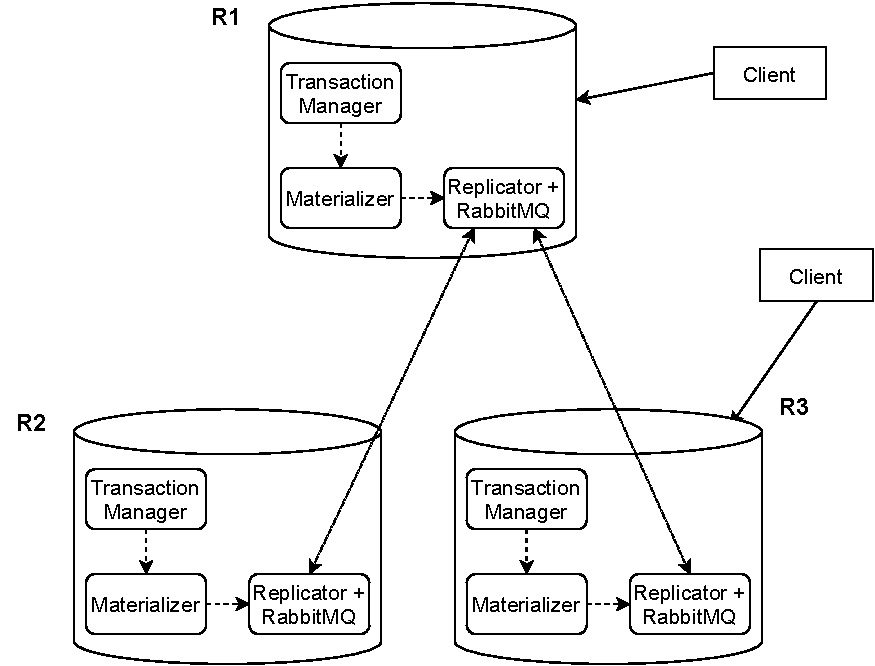
\includegraphics[width=.95\linewidth]{potiondb_architecture}
	\caption{PotionDB Architecture}
	\label{fig:potiondbArch}
\end{figure}

PotionDB is a key-value, geo-distributed store as illustrated in Figure \ref{fig:potiondbArch}.
Clients communicate with one or more servers to execute their operations.
Transactions are executed locally in one server, with updates being propagated asynchronously to other replicas.

Each replica contains only a subset of the objects - the system admin defines which groups (buckets) each server replicates (see Section \ref{???}).
If objects are partitioned correctly according to an application's needs, each client should only need to communicate with one server to do his operations, as all the data relevant to a client should be in one server.
In the case of not all required data being in one server, the client will need to contact multiple and execute a transaction in each server.
Note that this case should be exceptional - in most cases views will be replicated in all servers, thus reducing the need to consult other servers.

\andre{Should I even mention Cure here, and if yes, what else should I say about it, mainly in terms of similarities/differences with PotionDB}

\andre{Maybe the figure reference should only be here?}

The internal architecture of each PotionDB replica is similar to Cure \cite{cure}.
Each PotionDB replica can be separated in three main components:
\begin{enumerate*}[label=(\roman*)]
	\item TransactionManager (TM), which is responsible for receiving and replying to client requests, attributing timestamps to transactions and forwarding operations to Materializer;
	\item Materializer (MAT) which stores the object and applies both local and remote read/write operations, ensuring parallel snapshot isolation while executing those.
\end{enumerate*}

\begin{itemize}
	\item TransactionManager (TM), which is responsible for receiving and replying to client requests, attributing timestamps to transactions and forwarding operations to Materializer;
	\item Materializer (MAT) which stores the object and applies both local and remote read/write operations, ensuring parallel snapshot isolation while executing those.
	Local updates of a transaction are forwarded to the replicator once the transaction finishes executing;
	\item Replicator + RabbitMQ is responsible for both propagating updates to other replicas as well as receiving them. Operations are replicated asynchronously. We give more details on the replication  mechanism in Section \ref{subsec:replication}.
\end{itemize}


%apresentar a arquitetura a nível geral.

%Explicar servidores, clientes, sincronização.

\section{Transactions over Partially Replicated Data}

%Garantias
	% Snapshot isolation
	% Read commited
%Modelo de Consistencia?
	%Modelo de consistencia no acesso às views (garantias do utilizador)

\section{Supporting Views}
\label{sec:views}

\andre{I ended up not mentioning the challenges of supporting views, but let me know if I should fit those somehow}

In this section we elaborate on the mechanisms we use in PotionDB in order to support views.
Namely, we detail how views are updated when a relevant object gets updated, how partial replication affects views and how we keep the storage overhead of views reasonable.

%\andre{Possible topics for this?}
%\begin{itemize}
%	\item "Introduction?" (challenges? As in Section \ref{sec:views})
%	\item NuCRDTs
%	\item Triggers
%	\item View distribution and transactions (that is, explain how we require views to be in every replica that contains base data relevant to the view + view updates are bundled in the same transaction as the base object update. Definitely needs a better title.)
%\end{itemize}
%
%\andre{Also check Section \ref{sec:views}... maybe most of it is okay/re-usable?}

\subsection{Triggers}
\andre{Please check for repetition/overlap with section \ref{subsec:viewAPI}}

When an object is updated, all views to which that object may be relevant must be updated as well.
Another concern is how updates to an object are converted into view updates, specially when considering that any object supported by PotionDB can be used as a view.
We leverage on the usage of triggers to deal with both concerns.

The intuition behind triggers in databases is to automatically do an action when a read or update to given object(s) happen.
Similarly to some relational DBs \cite{???}, in PotionDB we use triggers to automatically generate updates to views when related objects are updated.
In Section \ref{subsec:viewAPI} we presented the interface for triggers. In this section we focus on how they are used.

\subsubsection{Storage}

\andre{We likely need to refer in the replication section how we replicate triggers? }

We store triggers in PotionDB as plain objects, i.e., not as CRDTs.
They do not need to be handled as CRDTs since:
\begin{enumerate*}[label=(\roman*)]
	\item each trigger is immutable (it can not be modified after being created);
	\item we assume trigger names are unique and, thus, there will not be any concurrent add/remove of a trigger.
\end{enumerate*}
While the latter point may seem questionable, we believe it is a fair assumption as triggers will not be created commonly by the clients, as they are usually defined by system admins and often before the database is populated.
Triggers are replicated as explained in Section \ref{???}.

\subsubsection{Matching}

As shown on Section \ref{subsec:viewAPI}, triggers can either be specific to one object or generic and thus concern multiple objects.
Single-target triggers are stored in a map indexed by the trigger's source object key, type and bucket, thus allowing direct access when an object is updated.
On the other hand, generic triggers are stored in a different map indexed by the source object type, as well as the operation type that fires the trigger (both elements cannot be generic).
When an update happens, the entry which contains the triggers (if any) for the source object and operation type is fetched.
For each trigger in said entry, the regular expression of the key and bucket is tested with the key and bucket of the object being updated.
A view update is generated if both match.

\subsubsection{Update generation}

\andre{two questions: a) should the part of clients applying the triggers be in its own subsection; b) should I mention that in the future we intend for servers to apply the triggers?}

On startup, clients fetch the list of triggers from a replica.
When a client intends to update an object, the triggers are checked as described previously.
For all triggers that match, view updates are generated.
Both the original object's and all generated view's updates are grouped in the same transaction, thus ensuring PotionDB will apply all of them with the same logical clock.

Recalling the API presented in Section \ref{subsec:viewAPI}, all triggers have a source and a target (view).
The source operation defines which object(s) and operation fires the trigger, as well as any variables, while the view part defines the operation to be generated and to which object.
Any variables used in the source can be used in view operation.
When an update happens, the variables are replaced with the actual values.

\andre{Should I just use a figure/table for this example instead of the paragraph below?}

To exemplify, consider a trigger with a source counter identified by the triple (counter[0-9]*, bucket1, COUNTER) and the operation inc(c).
Consider also a topk view identified by the triple (topk1, bucket1, TOPK) and the operation add(counter[0-9]*, c).
The update inc(5) to the object (counter12, bucket1, COUNTER) would generate the update add(counter12, 5) to the topk view.

\subsection{View consistency}

As previously mentioned, view updates are grouped with the source object in the same transaction.
PotionDB ensures that in a replica, all the updates of a transaction become visible at one moment in time.
This implies that a client can not see a state in which an object has been updated in a replica but its views have not.

%However, this still leave the following questions open: %\emph{How does partial replication affect views? How
%\emph{How do we ensure all replicas of a view receive view updates, even if they do not replicate the base data?}
However, this still leaves questions related to how partial replication may affect view updating. Namely, on how it is ensured that views are kept up-to-date even if not all relevant objects to a view are replicated in one replica.

%\andre{For as long as the clients generate the view updates, we don't require for views to be replicated in every replica. Do I still mention this? This section makes a bit less sense with triggers on client side.}

%\andre{The only thing that makes sense for now is to explain how }

When a client wants to execute a transaction, all the operations are sent to one replica.
A replica ignores all operations concerning buckets it does not replicate. 
Thus if a client wants to manipulate objects which are scattered across multiple servers, the client must contact multiple servers and send a transaction to enough servers in order to ensure each object to be updated is replicated in at least one of those servers.
This limitation can pose a problem concerning view updating - if a server contains an object relevant to a view but said view is not replicated there, the view update would be discarded.

\andre{I should refer in future work/some other place that we plan to address this limitation (not supporting updates for objects not replicated locally)? Do we actually want to address it? If not, we should justify/defend it}.

One possible solution for this is to require every server to replicate views.
This can be easily achieved by having one or more buckets just for views and having all servers replicate those buckets.
With this, a server will never discard an update to a view.
Due to how replication works (see Section \ref{subsec:replication}), this also ensures that all servers will replicate view updates and thus have their views up-to-date.
We note that this requirement is not a limitation - in fact, given the expected use case of PotionDB, it would already be desired for views to be replicated everywhere in most cases.
Even so, the exact requirement to keep views up-to-date is ligther:
more precisely, what is required is for a view to be replicated in every server in which there may be objects relevant to the view.
This lighter requirement might be useful for cases in which the view doesn't concern data from the whole globe but instead, e.g., from one given country.

%16/03/21:
%Para a secção "Supporting Views":
%- Explicar NuCRDTs
%- Explicar como se actualizam as vistas
%- Triggers
%- juntar operações
%- Se for apresentar as dificuldades/desafios, fazer algo curto.
%- Não explicar a consistência aqui.

\subsection{Non-uniform CRDTs}

Non-uniform CRDTs \cite{Cabrita17Nonuniform} leverage on the fact that, for certain objects, not all of the object's data is necessary to answer queries.
E.g., in a topK, only the K elements with highest value are required to answer a query.
Thus, non-uniform CRDTs capitalize on this by only requiring those K elements to be replicated in every replica, which allows to reduce storage overhead.

Cabrita et. al. introduce the concept of non-uniform eventual consistency. 
The key difference between eventual consistency and non-uniform eventual consistency is that, instead of requiring for the states of each object to be eventually equivalent, it requires for the \emph{observable} stables to be eventually equivalent \cite{Cabrita17Nonuniform}.
Two states are defined as observable equivalent iff, for each possible query, the result is equivalent when executed on either states.
This allows to save both storage space and communication overhead, as not all updates in a non-uniform CRDT must be replicated to all replicas \cite{Cabrita17Nonuniform}.

Non-uniform CRDTs are specially useful to serve as materialized views, as they allow to keep summaries of data easily while also being space-efficient.
E.g., if we consider the scenario described in Section \ref{sec:example} and a topK of ``top 100 consumers who spent the most'', even if there's millions of customers globally, each replica does not need to keep data for all customers in order to correctly apply reads in the topK CRDT.

PotionDB fully supports the usage of NuCRDTs for its objects.
Thus, when an operation is applied on a NuCRDT object, the operation is only replicated to all of that CRDT's replicas iff that operation changed the visible state.
Some operations however may only have an effect later (e.g: in a topK, an element may rise to the top after another one gets removed) \cite{Cabrita17Nonuniform}.
Operations in that category are only replicated from one replica to the others when it affects the visible state.

\andre{Should I specify, *clearly*, that all replicas "together" need to keep the whole CRDT state? As in, if we concatenated the state of each replica, we would get the full state. I already hint this in the previous paragraph.}

\section{Partitioning, Replication and Consistency}

%In this section we discuss three important design decisions in PotionDB:
In this section we describe important mechanisms in PotionDB: partitioning, replication and transactions.
The referred mechanisms are the basis for efficiently supporting queries on global data, while maintaing reasonable update performance and space overhead.

\subsection{Partitions}

\andre{I've decided to, for now, use here the terms partition/sharding for, respectively, internal \& external partitioning. Maybe I should do the same in previous sections (namely Section 4)?}

In PotionDB objects are partitioned both internally in a server and externally between different servers.
Internally, we partition in order to efficiently utilize multicore CPUs, while externally we partition to reduce the amount of data stored and processed in each server, making usage of data locality.

To simplicify, we refer to external and internal partitioning as, respectively, sharding and partitioning.
We now explain how both mechanisms work in PotionDB.
%Both partitioning mechanisms work differently and have different goals, which we explain in this subsection.

\subsubsection{Partitioning}

In a PotionDB instance, objects are split across multiple partitions.
Each partition has one thread associated to it, which allows requests in different partitions to potencially be processed in parallel. 
Each object is assigned to one partition automatically, based on a hash of the composition of the object's key, bucket and type.
%Inside a server objects are split across multiple partitions.
%Each object is assigned to one partition automatically.
%The partition to which an object is assigned to is determined by computing an hash based on the object's key, bucket and type.

The intuition behind partitioning objects in a server comes from the observation that, by having data grouped in multiple ``slots'' (i.e., partitions), if different clients access objects in different partitions, then both requests can be processed in parallel by a replica without any conflict.
And if both requests are read only, they can be processed in parallel even if some objects are present in both requests, as reads don't conflict \cite{???}.

At a first glance it may seem odd to partition based on a hash with the goal of improving performance.
However, this is justified by the expected use of PotionDB - simirlarly to relational databases, the most frequent and complicated queries are expected to have, for each one, a single view that answers them directly, thus requiring only a single operation.
Due to the nature of hashing, these views are likelly to be spread across multiple partitions.
This implies that multiple queries can be executed concurrently without conflicts even in the presence of concurrent updates that only affect unrelated objects.
Our practical evaluation shows that this partitioning improves PotionDB's performance quite considerably. \andre{Does it actually show that? Should we show that?}
%TODO: This very likelly won't be included in the Practical evaluation section. I may have to run some benchmarks and report the results here.

\andre{What's below is probably not needed. It's just a comparison with other alternatives}

%A possible alternative to internal partitioning and still make use of multi-core CPUs would be to use locks to control access to the same object, in order to prevent write conflicts \cite{???}.
Other possible solutions to make use of multi-core CPUs are possible, for instance:
\begin{enumerate}
	\item \label{item:locks} using locks to protect the same object from being concurrently modified \cite{???};
	\item \label{item:multiplePotion} running multiple PotionDB servers in the same computer.
\end{enumerate}

%In theory this can lead to a considerate performance improvement, as each replica can make use of their multi-core CPUs by having one thread per partition to process requests.
%Other possible solutions include: 
%\begin{enumerate*}[label=(\roman*)] 
	%\item \label{item:locks} using locks to protect the same object from being concurrently modified \cite{???};
	%\item \label{item:single} using only a single thread \cite{???}.
%\end{enumerate*}

Alternative \ref{item:locks} is difficult to implement, as it is required to find the right level of lock granularity and when should locks be obtained/released \cite{???}. 
Special care is needed to avoid deadlocking concurrent transactions. 
There's also concerns with both fairness and overhead of obtaining locks.
Our solution does not need to lock data, thus it avoids the overhead from using locks, is easier to implement and does not have deadlocks.

As for \ref{item:multiplePotion}, this would imply more replicas running in the system, which increases both replication and storage costs.
This would also imply concurrency conflicts even in the same computer.
Finally, while this can allow more clients to be processed in the same period of time, and is quite easy to implement, it does not improve the performance of each client, as each transaction must be done in a single replica (and thread) to avoid breaking consistency. \andre{Does this need to be explained? The idea here is that we would lose the "write follows reads/writes" property.}

%As for \ref{item:single}, the solution does not take any benefict from  the multiple cores of nowadays CPUs \cite{???}. In section \ref{???}, we show that this solution has worse performance than ours, specially with read-only transactions.

\subsubsection{Sharding}

\andre{This has a lot of overlap with Section \ref{subsec:databasemodel}}

Since PotionDB is a partially replicated \cite{???} database, it is necessary to have a mechanism which allows to precisely define in which servers should an object be replicated in.

We achieve this by requiring each object to be identified not only by its key, but also by a ``bucket''.
Buckets define groups of objects that are replicated in the same group of replicas. In other words, two objects with the same bucket value will be replicated in the same set of replicas.
For each replica, the system admin can define which buckets will be replicated in it.

To exemplify, recall the commerce example presented in Section \ref{sec:example}.
The customers can be partitioned based on their country's continent by taking the following steps: 

\begin{enumerate}
	\item Define one bucket per continent;
	\item Configure the servers so that each replica replicates the bucket of its continent + another one for fault tolerance purposes;
	\item When adding a customer to the database, specify the bucket correspondent to the customer's continent.
\end{enumerate}

%PotionDB's replication mechanism takes in consideration the bucket distribution among servers, ensuring only servers interested in a given bucket receive updates for that bucket.
It's worth noting that clients must ensure they are communicating with a server which replicates the buckets they want to operate on, since each server only replicates a subset of the buckets and doesn't forward operations to other servers.

\subsection{Replication}
\label{subsec:replication}

\andre{Note: If we decide to keep this section, maybe I should add a scheme showing each server "subscribing" buckets and another with the operations being sent? Also now that NuCRDTs were moved to Section \ref{sec:views}, we likely need to rethink what should be explained here.}

%Explain the basic idea of replication (async, partial, etc). Also include NuCRDTs here.
Replication in PotionDB is asynchronous and partial.
Operations are executed localy, without needing to contact other replicas.
Periodically, new updates are propagated asynchronously to other replicas.
All objects in PotionDB are operation-based CRDTs, thus the information required to propagate an update consists in the operation type and its arguments.

\subsubsection{RabbitMQ}
\label{subsubsec:rabbitmq}

PotionDB uses RabbitMQ \cite{???} for handling communication between replicas.
RabbitMQ is a message brooker which allows consumers to register the topics of messages in which they're interested.
We leverage on topics to ensure each replica only fetches the messages containing updates for objects in buckets they are replicating.

We use RabbitMQ as follows.
Each PotionDB server runs alongside it a RabbitMQ instance.
When a replica starts, it contacts other server's RabbitMQs and subscribes to all messages whose topics match the buckets it replicates.
When a replica wants to publish new updates, it splits those updates by buckets (while maintaining causality), ensuring each message only contains updates for one bucket and whose topic value is that bucket.
Those updates are then sent to the local RabbitMQ instance, which then forwards them to interested PotionDB instances.
A receiving replica then rebuilds the transactions, applying the transaction once every update (for the buckets it replicates) of a transaction is received.
Causality related transactions will be applied according to their original order.

We also use RabbitMQ to support the addition of new replicas without stopping the system.
However, such mechanism is outside of the scope of this paper and thus we don't describe it here.

%\subsubsection{NuCRDTs replication}
%\label{subsubsec:nureplication}
%
%Non-uniform CRDTs \cite{Cabrita17Nonuniform} leverage on the fact that, for certain objects, not all of the object's data is necessary to answer queries.
%E.g., in a topK CRDT that only maintains the K elements with highest value, only those K elements must be replicated in every replica.
%
%The key difference between eventual consistency and non-uniform eventual consistency is that, instead of requiring for the states of each object to be eventually equivalent, it requires for the \emph{observable} stables to be eventually equivalent \cite{Cabrita17Nonuniform}.
%Two states are defined as observable equivalent iff, for each possible query, the result is equivalent when executed on either states.
%This allows to save both storage space and communication overhead, as not all updates in a non-uniform CRDT must be replicated to all replicas \cite{Cabrita17Nonuniform}.
%
%Non-uniform CRDTs are specially useful for using as materialized views, as they allow to keep summaries of data easily while also being space-efficient.
%E.g., if we consider the scenario described in Section \ref{sec:example} and a topK of ``top 100 consumers who spent the most'', even if there's millions of customers globally, replicas don't need to keep data for all customers in order to correctly apply reads in the topK CRDT.
%%E.g., in the scenario described in Section \ref{subsubsec:APIView}, even if there's millions of customers globally, replicas don't need to keep data for all customers in order to correctly apply reads in the Top-K CRDT.
%
%\andre{What's above, technically, isn't 100\% true: all replicas together need to keep ALL entries of the top-k due to removes being supported. Thus, an entry for all customers in the system. However, no single replica needs to keep all entries.}
%
%PotionDB fully supports NuCRDTs.
%Thus, when an operation is applied on a NuCRDT, the operation is only replicated to all of that CRDT's replicas iff that operation changed the visible state.
%Some operations however may only have an effect later (e.g: in a topK, an element may rise to the top after another one gets removed) \cite{Cabrita17Nonuniform}.
%Operations in that category are only replicated to all replicas when it affects the visible state.
%
%\andre{Should I refer that those operations in the last category are/should (as they aren't as of now) be sent to a few replicas for fault-tolerance purposes?}

\subsection{Transactions}

\andre{This section quite likely still needs to be heavily worked on, but I don't know how to proceed with it...}
%Somehow explain that we'll cover casual consistency/PotionDB's consistency guarantees in the transactions subsubsection.

PotionDB offers transactions with casual consistency.
That is, clients see operations' effects by an order consistent with causality \cite{???}.
%Probably cite lamport or similar
Since casual consistency is a form of weak consistency, concurrency conflicts will still occour when operations are applied on different replicas.
We leverage on CRDTs in order to deal with those.

%We now describe in more detail which guarantees our transactions provide, as well as how we keep views and their base objects in sync.
Transactions allows to group multiple operations together and have them executed with certain guarantees.
They facilitate the usage of database systems \cite{???}.
For example, when registering a sale of a product, it is useful to have the product stock and customer info to be updated simultaneously. %TODO: We might need a better example

Relational databases typically provide ACID (atomicity, strong consistency, isolation, durability) guarantees for their transactions \cite{???}.
These properties ensure that, respectivelly:
\begin{enumerate*}[label=(\roman*)]
	\item either all operations execute successfully or none does;
	\item the database is left in a consistent state;
	\item there is no interferance from other transactions;
	\item the effects of the operations won't be lost even if replicas fail.
\end{enumerate*}
Having all of these properties facilitates the development of applications, as it reduces the possible anomalities that may be observed.
E.g., in the scenario of a cash transfer between two entities, if we forego atomacity, it's possible the cash is withdraw from one account without being deposited in the other due to, e.g., a server crash.

Unfortunately providing ACID in a database requires providing strong consistency \cite{???}
%TODO: I need to find sources for this
, which implies reduced fault tolerance and may limit performance.
In a geo-distributed scenario it also implies a quite higher latency overhead due to the required synchronization between DCs \cite{???}.
Transactions are still useful even without all ACID guarantees, as is evidenced by multiple weakly consistent databases providing them with different guarantees \cite{???}.
%TODO: This might need an example

PotionDB supports non-ACID transactions.
Transactions in PotionDB can span any number of partitions (both internal and external) existent in a replica, but it cannot refer to buckets that aren't replicated locally.
That is, transactions are local to a replica.
We support both read-only, write-only and mixed transactions, with all having the same guarantees.

PotionDB's transactions are atomic and provide causal consistency.
Each transaction runs isolated from other transactions in the same server, but the same objects may be concurrently modified by different transactions in different servers.
Durability isn't ensured, as replication is asynchronous and operations don't need to be written to disk for a transaction to commit.
In order to understand in detail the guarantees of PotionDB's transactions, some insight on how they're handled needs to be given.

\andre{We don't exactly guarantee atomicity - if the replica executing the transaction fails while applying updates, the DB will be left in an inconsistent state. Which isn't exactly relevant, since data would be lost in that case anyway... We do guarantee that, if the server doesn't fail, the client either sees the effect of the whole transaction or of none of its operations.}

\andre{Also... how much detail of the transaction execution mechanism should I provide here? Or just talking about the guarantees is enough?}

Each replica maintains a vector clock which summarizes the current DB state.
Each entry in the vector clock corresponds to the latest commit of each replica that is known locally.
When a transaction starts, a copy of this vector clock is associated to the transaction.
The entry correspondent to the local replica is processed differently - for that entry, a unique, monotonically increasing timestamp, is assigned to each transaction, which ensures each transaction will commit with a different vector clock.

\andre{Where (and should I?) do I explain how the version management works? Or should we leave that for a short paper in another conference? Also I'm hiding the 2 phase-commit part, and that commitTS != initialTS.}

Both updates and reads take the transactions' vector clock into account.
More precisely, reads execute on the state of the object correspondent to the transaction's vector clock (i.e., ignoring all update operations that may have happened afterwards, but considering updates in the same transaction that happened-before).
The effects of updates are only applied to the latest-version of an object when the transaction is commiting.
Transactions commit according to the order defined by the vector clocks.
A transaction is considered commited after all operations have been applied.
%Updates generate new states which are then marked with the transaction's timestamp, in order for reads to refer to the correct version.
%A transaction is considered commited only after all operations have been applied. 
At this moment, if it isn't a read-only transaction, the replica's entry on the local vector clock is updated and the client is notified.

%PotionDB's guarantees in regard to transactions are related with how the vector clock is handled. More precisely:
We can now leverage on the workings of PotionDB's transactions to detail the exact guarantees they provide.

%E.g., in a read-only transaction, even if some update operation concurrently modifies objects referred by the read transaction, the results returned by reads will all be using the version specified by the transaction. That is, it is as if the update operation happened after the reads.

\paragraph{Atomicity}  A transaction is atomic because the replica's vector clock is only updated after all operations are successfully applied. 
If at least one fails, all updates are rendered innefective as we return the CRDTs to their previous state.
Previous reads on that transaction are irrelevant due to the transaction being considered as aborted.
Reads on other transactions don't see the effects of a transaction until it is commited, thus aborts don't pose a problem to them.
Other replicas only start applying a transaction after all updates for it are received.

\paragraph{Consistency} As every transaction has a vector clock associated, we can thus totally order all transactions. 
A transaction is only executed if all transactions with a smaller vector clock have already been executed. 
We ensure locally generated transactions are executed by the order specified by the monotonicaly increasing local timestamp.
For concurrent transactions any order is possible and consistent with casual consistency.
CRDTs ensure concurrent operations don't pose a problem as they're commutative \cite{???}.
Whenever a CRDT is about to be updated, all of its matching triggers are executed and the resulting updates are included in the same transaction with the same clock.
%Whenever a CRDT with views associated is updated, the views are also updated in the same transaction with the same clock.
Thus, PotionDB respects causality when executing transactions and, as such, provides causal consistency.

\paragraph{Isolation} %During the execution of a transaction, reads and updates are all executed on top of the version specified by the transaction's vector clock.
%Inside each partition there is no concurrency and all of a transaction's operations are executed in a row
There is no concurrency inside each partition.
Reads are executed on top of the version specified by the transaction's vector clock. %TODO: Should I refer here that txn updates are considered for the read albeit they don't change the state yet?
Updates are only applied when commiting and are executed sequentially inside the partition.
Updates from other transactions are either executed before the first operation of the current transaction, or after the last.
Thus, the effects of each local transaction can be ordered sequentially, which implies isolation.
We do not guarantee isolation between transactions executing in different replicas however.

It is important to note that even though we provide atomicity, consistency and isolation guarantees, the latter two are not equivalent to the ones provided in ACID.
We provide causal consistency (i.e., weak consistency) instead of strong consistency; we don't guarantee isolation between servers (which is required in ACID).
As evidenced in both academy and industry, while ACID properties are quite useful, they are also quite limiting in terms of fault tolerance and performance \cite{???}.

\section{Views}
\label{sec:oldviews}

Views are useful as they make it easier to specify queries and, in the case of materialized views, it may improve their performance as well.
An essencial question in supporting materialized views in a database is on keeping them coeherent with the base data they refer to.
When an object is updated the views must also be updated, otherwise the database becomes inconsistent which may then lead to errors in applications \cite{???}.

Usually in relational databases, views are updated automatically by using triggers associated to the base data tables \cite{???}.
Due to data being fully replicated and strongly consistent, it is guaranteed that at all times the view reflects the latest correct state \cite{???}.

PotionDB also uses triggers to keep the views updated. However, as PotionDB is a weakly consistent, geo-distributed and partially replicated database, extra challenges are imposed for maintaining materialized views up-to-date, namelly:
\begin{enumerate}
	\item Association between views and their base data. 
	PotionDB is a key-value store, thus multiple objects that would usually belong to the same table in a relational database (e.g., customers) have different keys associated.
	\item Automatic inclusion of objects created after the view that represent entities of the same kind (e.g., new customers) but necessarely have different keys.
	\item Translation of updates in base data to views. 
	Unlike in relational databases in which all data can be seen as tables with multiple columns, here there are multiple types of objects which have different kinds of properties and operations.
	\item Keeping the views and base data synchronized at all time.
	I.e., from the perspective of a client, updates on base data should lead to the view being updated simultaneously.
	%This isn't a problem in relational databases as they will belong to the same table.
	\item Keeping views updated even if all necessary data for it isn't present locally due to partial replication.
\end{enumerate}

In this section we detail the inner workings of views and triggers, and show how we address the points referred above.
We start by explaining what we define as a view, how are triggers used and updates generated for the views.
We end with discussing how our replication mechanism ensures view updates are sent to every replica that replicates those, even if they don't replicate the relevant base data.

\subsection{View CRDTs and Triggers}

We define as a view CRDT any CRDT that is updated automatically based on updates to other existing CRDTs.
To define how views should be updated, we leverage on the concept of triggers.

A trigger defines how updates on an object (source) translate to updates on another object (view).
The API was already described in Section \ref{subsubsec:APIVew}, thus in this section we focus on how triggers work internally.

\paragraph{Storage}We store triggers in PotionDB as special objects.
They do not need to be stored as CRDTs, as:
\begin{enumerate*}[label=(\roman*)]
	\item each trigger is immutable (it can not be modified after being created);
	\item we assume trigger names are unique and, thus, there won't be any concurrent add/remove of a trigger.
\end{enumerate*}
While the latter point may seem questionable, we believe it is a fair assumption as triggers will not be created commonly by the clients, as they are usually defined by system admins and often before the database is populated.
Triggers are replicated as explained in Section \ref{subsubsec:rabbitmq}.

\andre{Maybe the claim above needs a citation? Suggestions?}

\andre{Note: The storage description above is how I expect to implement it in the near future. At the moment clients store the triggers, but the next step will be for the servers to store them (clients will then have to fetch them)}

\andre{I probably need a better title for the paragraph below. Suggestions?}

\paragraph{Clients apply triggers} When a client starts, the existing triggers are fetched from the database, and stored on the client.
Then, whenever a client requests an update, it checks its triggers in order to generate the appropriate updates for the views.

\paragraph{Matching} As explained in Section \ref{subsubsec:APIVew}, triggers can either be specific to one CRDT or generic (i.e., match with multiple source CRDTs).
Non-generic triggers are stored in a map whose key is the uid (key, bucket, crdtType) of the source CRDT.
Thus, non-generic triggers can be directly indexed when an update to a source CRDT is issued.
On the other hand, for generic triggers, we index them by CRDT and operation type, as both the key and the bucket may be regular expressions.
For a given update, every trigger whose CRDT and operation type is equal to those of the update, is tested to see if the key and bucket respect the regular expressions and, thus, a view should be updated.

\paragraph{Update generation}
Each trigger contains both a source operation and a view operation, which are relative to, respectively, the source and view CRDTs.
On the source operation we can define variables that will then be used on the view operation. E.g., if the source operation is \emph{inc(c)}, the 'c' is a variable that can then be used in the view operation, e.g., \emph{add('id1', c)}.
When an operation is prepared, the variables are replaced by their respective values, e.g., \emph{inc(5)} gets translated into \emph{add('id1', c)}.
Updates generated by triggers are added to the same transaction of the initial update, thus ensuring both updates to views and base data become visible at the same time.

\subsection{Implications of partial replication  on views}

%We now explain how views in PotionDB don't require all of its base data to be present in the same server as the view. To demonstrate this, we will first assume one of the servers contains all the base data for a given view, and then drop such assumption.
We now explain what are the implications of partial replication in PotionDB's views and, more precisely, how does replication need to be configured in order for views to work properly.

For now, we will assume that there is one server (PotionDB1) which contains all the base data that may be used to generate a given view.
If the clients always contact PotionDB1 to update such base objects, and thus the view, PotionDB's replication mechanism would ensure that all replicas which replicate the view's bucket would receive its updates (see Section \ref{subsubsec:rabbitmq}).
Since updates are sent separately, grouped by bucket, other replicas will receive the view updates as long as they replicate the view's bucket, even if they don't replicate the respective base data.
Thus, we have concluded that it is not necessary for every replica to replicate the base data of a view, as long as one server has all the base data.

We now drop the assumption that one server has all the base data, assuming instead that all relevant data is split across multiple servers.
Assuming that when a client wants to update one of the base objects, the contacted server (PotionDB2) replicates such object, we have two scenarios:
\begin{enumerate*}[label=(\roman*)]
	\item PotionDB2 replicates the view and, thus, both updates to base data and view are applied and replicated to other replicas (as described previously);
	\item PotionDB2 doesn't replicate the view, thus updates to the view are ignored, as we require that clients send their updates to servers which replicate the referred buckets.
\end{enumerate*}
In short, whenever a base object is updated, as long as such server also replicates the view's bucket, both the base object update and view's will be replicated to the relevant servers.

With this, we can now define how replication must be configured in order for views to work correctly.
The simpler solution is to have a special bucket for views, which is replicated in every server.
This ensures some server will always have any data that may be relevant to the view.
However, the precise requirement is that a view's bucket must be replicated in every server that contains, or may eventually contain, objects relevant to such view.

We note that it would be possible to ease this requirement further if the clients send updates of base data and views to different servers, as in this case one single server replicating the view would be enough, even if such server had none of its base data.
However, this would imply that the update of the view and of the base data would not be in the same transaction.
This in turn has the downside of, in servers which replicate both the view and some of its base data, to have the updates of the view and base data applied at different times, thus possibly giving an inconsistent representation of the database to the client for a certain period of time.

%Explain how it isn't necessary to have all data replicated everywhere, and how it suffices to have views replicated in every replica in which there may be a relevant base data.
%

%Explain how triggers are stored and used
	%Server stores them on a special object; clients fetch triggers; clients generate view updates
%Explain the update procedure on clients
	%Prepare main update; check non-generic triggers; check generic triggers; send all updates
%Address points 4 and 5 - same transaction; bucket mechanism ensures view updates are sent to every replica.

\section{Implementation}

\section{Evaluation}

In this section we conduct multiple experiments in order to evaluate PotionDB's performance.
Namely, we try to assess the advantage of all replicas having views spanning data partitioned across multiple replicas, instead of each replica having an incomplete view with only its local data (local PotionDB).
E.g., if we partition customer's data based on the continent of the customer's country, the local view of a server in Europe would only concern the data of european customers, while a global view would include customers from all over the globe.
We also compare PotionDB with a solution that has one server dedicated to host all indexes (single index PotionDB).

\subsection{Settings}

\subsubsection{Common settings}

For our tests, we use a dataset based on TPC-H's dataset \cite{tpch}.
More precisely, while we keep all the tables and use data generated by the dbgen tool \cite{tpch}, we focus only on a subset of the queries and, for each table, we only keep the columns necessary for such queries.
We also use the following settings in common across all of our tests:

\begin{itemize}
	\item Five PotionDB instances, each one executing in its own node.
	Each node has a AMD EPYC 7281 CPU with 96GB of RAM, with PotionDB only being able to use 8 cores of the CPU (this helps ensure the bottleneck is not on the client side); \andre{Should I keep this?}
	\item Each PotionDB instance replicates the data of a continent, e.g., a server replicates all data concerning Europe while another keeps the data of Asia. Data that isn't location based such as products is replicated in all servers, as are indexes.
	\item Servers are interconnected by a LAN with 10 Gbps speed;
	\item Clients execute on nodes with 2x Intel Xeon E5-2620 v2 CPU and 64GB of RAM, being on the same LAN as the servers but with a reduced network speed of 1Gbps;
	\item Each client selects one server to execute queries upon, only contacting other servers if all the data required to reply to a query isn't present in the selected server. \andre{Should I refer that, in practice, this only happens in the local views scenario?} By default, the queries executed are 3, 5, 11, 14, 15 and 18 of the TPC-H specification \cite{tpch};
	\item Unless otherwise specified, each request only executes one query or updates one sale (including all related indexes).
\end{itemize}

All our experiments execute as follows.
First, all servers are started, with each one estabilishing a connection with all others.
Afterwards, a special client is started to load the initial database state into the servers, taking into consideration the locality of the data.
%Finally, after all data has been loaded into the servers, multiple clients are started to execute queries.
%In some tests, a client responsible for updating the dataset (i.e., insert new elements and remove old ones) is also started along with the query clients.
%We call this last client of update client.
%In some other tests, all clients can do both queries and updates, with a varying percentage.
Finally, after all data has been loaded into the servers, multiple clients are started to execute queries and, possibly, updates, with the query/update rate depending on the test.

In our experiments we use as metrics the amount of operations per second (ops/s) achieved by all clients aggregated, as well as the average latency of each client request.
To determine how much each test can scale, we vary the number of clients.
As the number of clients increases, so does the latency of each request and, until the servers saturate, the throughput of the servers.

\subsubsection{Scenarios}

We make an extensive evaluation of PotionDB, conducting multiple experiments in order to evaluate how PotionDB scales in different scenarios. %When appropriate, we also execute the same experiments for local PotionDB and single index PotionDB.
%With these experiments, we try to assess the following:
With these experiments, we try to answer the following:

%\begin{itemize}
%	\item How does PotionDB compare with other solutions, namely the local and single versions of PotionDB? How does the data locality and size affect the performance?
%	\item How much is PotionDB able to scale when executing queries only, or when trying to execute both queries and updates simultaneously?
%	\item How does different read/write ratios affect PotionDB's performance?
%	\item How well does each CRDT type scale in PotionDB, namelly when its size grows?
%\end{itemize}
\begin{enumerate}
	\item \label{enum:question1} What is the practical benefict of having views of data replicated across different servers, compared to having only views of local data (local PotionDB) or a single index server (single PotionDB)?
	\item \label{enum:question2}What is the effect on PotionDB's throughput of executing updates, namely as the write/read ratio increases?
	\item \label{enum:question3}How much can PotionDB scale if we group operations?
	\item \label{enum:question4}\andre{TODO: benchmarks}
\end{enumerate}

\subsection{Results}

\subsubsection{Locality of data}

\andre{I wonder if it's worth mentioning that the number of clients server in single/local versions is much lower compared to normal.}

To evaluate the benefits of having indexes replicated in every replica (\ref{enum:question1}), we compare PotionDB with the local and single versions, namely in terms of queries per second.

\begin{figure}
	\centering
	\begin{subfigure}{.5\linewidth}
		\centering
		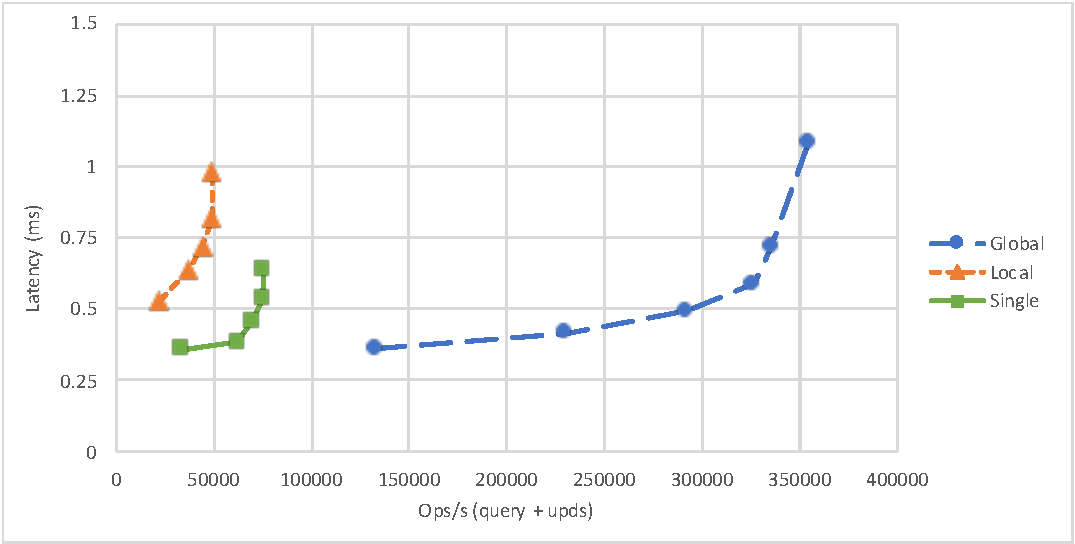
\includegraphics[width=.95\linewidth]{global_local_single_cut}
		\caption{All queries}
		\label{fig:global_local_single}
	\end{subfigure}%
	\begin{subfigure}{.5\linewidth}
		\centering
		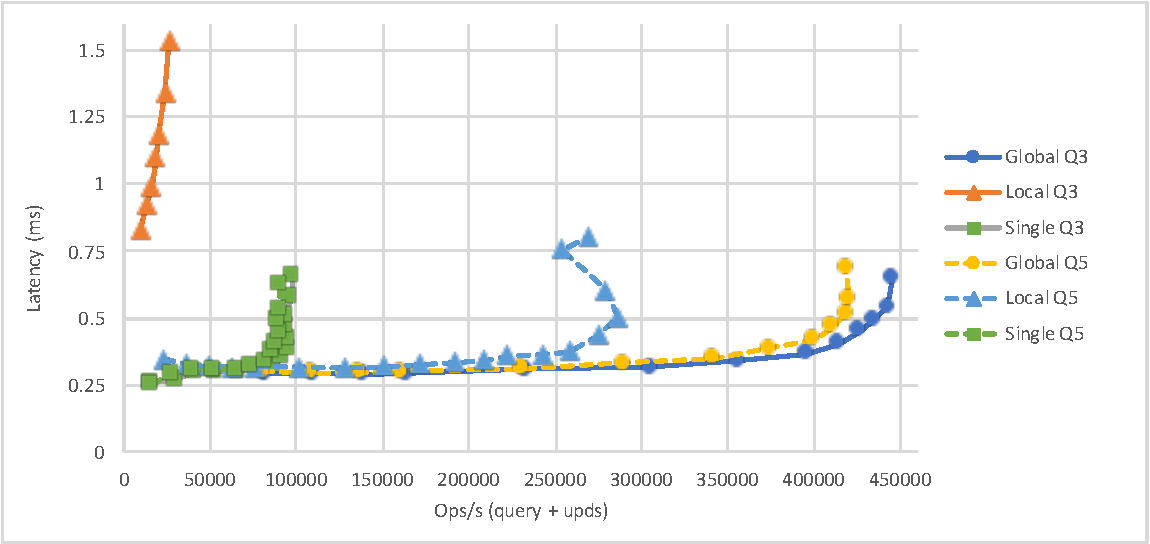
\includegraphics[width=.95\linewidth]{individual_query_cut}
		\caption{Single query type}
		\label{fig:q3q5}
	\end{subfigure}
	\caption{Query-only performance of PotionDB and its local and single index versions. On the left all queries are executed, while on right it is only Q3 or Q5.}
	\label{fig:query_only}
\end{figure}

Figure \ref{fig:query_only} shows the results of experiments for the three versions of PotionDB, in terms of query/s versus latency.
Figure \ref{fig:global_local_single} includes all queries in the execution, while \ref{fig:q3q5} only includes a single type of query at a time.

As expected, on both cases the performance of the local and single versions is worse than normal PotionDB.
Focusing on figure \ref{fig:global_local_single}, it is noticeable that local version performance is about 7 times lower than normal.
This happens because most queries require data from all regions, thus requiring local clients to contact all servers and wait for them all to reply.
This leads to both more load on each server as well as more time waiting on the client side.
The single scenario performance is roughly 1/5 of normal's.
This can be explained as all queries only need to consult the indexes, which due to those being all in one server, implies that the load is all directed to one server instead of being split across five.

Figure \ref{fig:q3q5} shows that the lower throughput of the local version is due to the locality of the data - Q3 requires data from all servers and has about 1/12 of the performance of normal PotionDB, while Q5 only requires data from one region (thus one server) and has about 2/3 of the performance.
This smaller drop can be explained due to local clients not being sticky - as the query parameters are selected at random, local clients are forced to constantly query different servers, while each normal client can query always the same server.

\subsubsection{PotionDB scaling - queries VS updates}

We now evaluate the impact on PotionDB's throughput of executing updates alongside queries, with multiple read/write ratios (\ref{enum:question2}).
In this scenario, whenever a client wants to execute an operation, it picks at random whenever a query or an update is executed.
It is worth noting that an update affects both base data and all associated indexes.
Also note that while index updates are executed in every replica, we only count them once (i.e., if one update is executed 5 times, it still only counts as 1 operation).

\begin{figure}
	\centering
	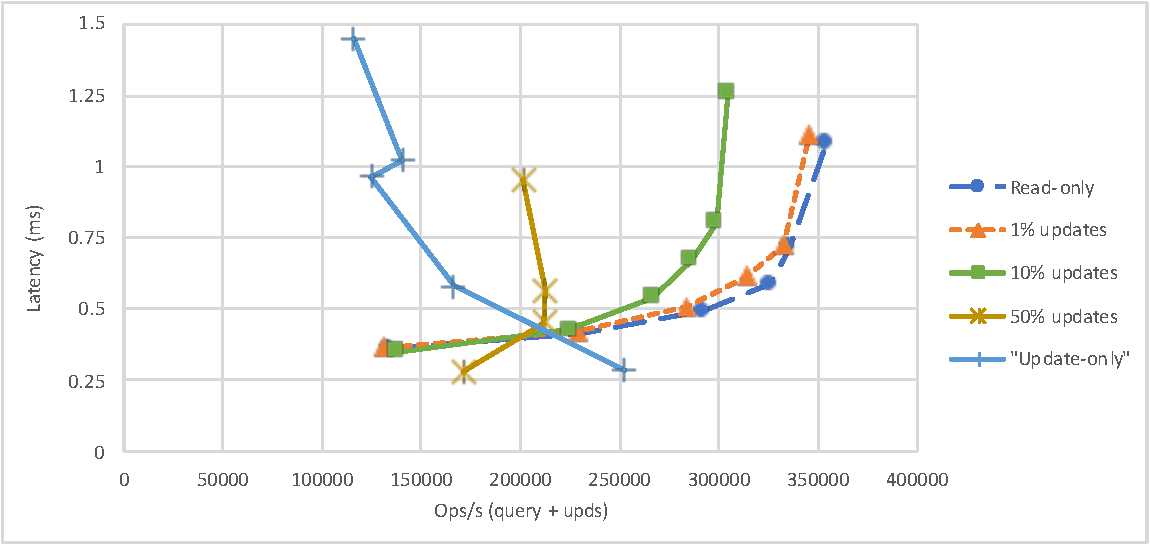
\includegraphics[width=.95\linewidth]{update_rates_cut}
	\caption{PotionDB performance with varying update rate.}
	\label{fig:update_rates}
\end{figure}
\begin{figure}
	\centering
	\begin{subfigure}{.5\linewidth}
		\centering
		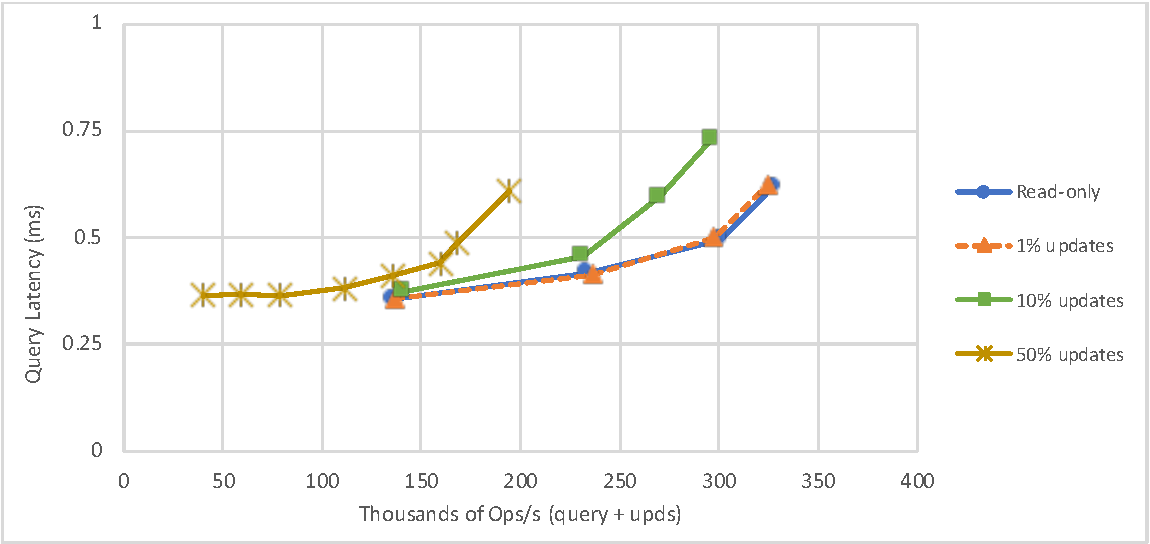
\includegraphics[width=.95\linewidth]{update_rates_query_cut}
		\caption{Query-latency}
		\label{fig:update_rates_query}
	\end{subfigure}%
	\begin{subfigure}{.5\linewidth}
		\centering
		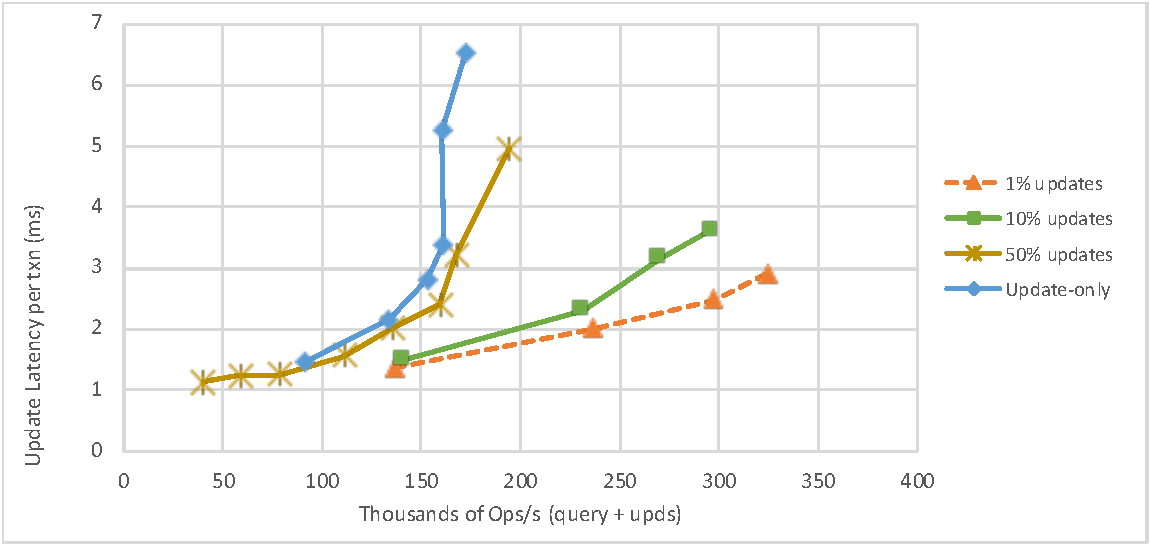
\includegraphics[width=.95\linewidth]{update_rates_update_cut}
		\caption{Update-latency}
		\label{fig:update_rates_update}
	\end{subfigure}
	\caption{PotionDB performance with varying update rate, with query and update latencies split. Note that updates are done in groups due to having to update both base data and indexes.}
	\label{fig:update_rates_split}
\end{figure}

Figure \ref{fig:update_rates} shows the results of executing updates alongside queries, with varying odds of choosing an update.
For low update rates (1\% and 10\%), the decrease in performance can be considered reasonable (aproximately 2,5\% and 14\%).
For higher rates, two observations can be made:
\begin{enumerate*}[label=(\roman*)]
	\item the servers saturate earlier, in some cases even decreasing throughput as the number of clients rises;
	\item the max throughput is lower.
\end{enumerate*}

The referred observations can be explained if we consider the following. 
With PotionDB's internal partitioning, queries on different objects can be executed concurrently, thus query-only scenarios scale easily. 
However, updates in a transaction must lock the partitions they're involved and do a 2-phase commit, in order to ensure the states evolve sequentially in a replica even when concurrent transactions are issued.
As such, if the update rate is high, clients executing queries or updates may often have to wait for a transaction with updates to finish executing before executing their own operations.
\andre{I might have to reffer in an early section with more detail how we do updates in our experiment, namely that our granularity is at order-level and that indexes, orders and items are updated in the same txn.}.

Figure \ref{fig:update_rates_split} shows the same experiment as figure \ref{fig:update_rates}, but showcases the latencies of queries and updates splitted, instead of together.
It is noticeable that updates have quite higher latencies and scale much less, which is due to both 2-phase commit and grouping of operations (as updates need to be reflected on both base data and indexes).


\andre{Probably some concluding note that reffers that for PotionDB's intented usages it is likely that updates are much less frequent than queries, or maybe even that updates could maybe be delayed?}

\subsubsection{Batching}

On the previous scenarios, each client only requested one query at a time, even through updates were executed in groups (whenever one update to a base object is usued, all associated indexes are updated in the same transaction).
With this we've noticed that, with a low number of clients, an update-only scenario actually has better throughput than a query-only scenario.
Thus, we now evaluate the effect observable on PotionDB's throughput if multiple queries are included in the same transaction (\ref{enum:question3}).

%\begin{figure}
%	\centering
%	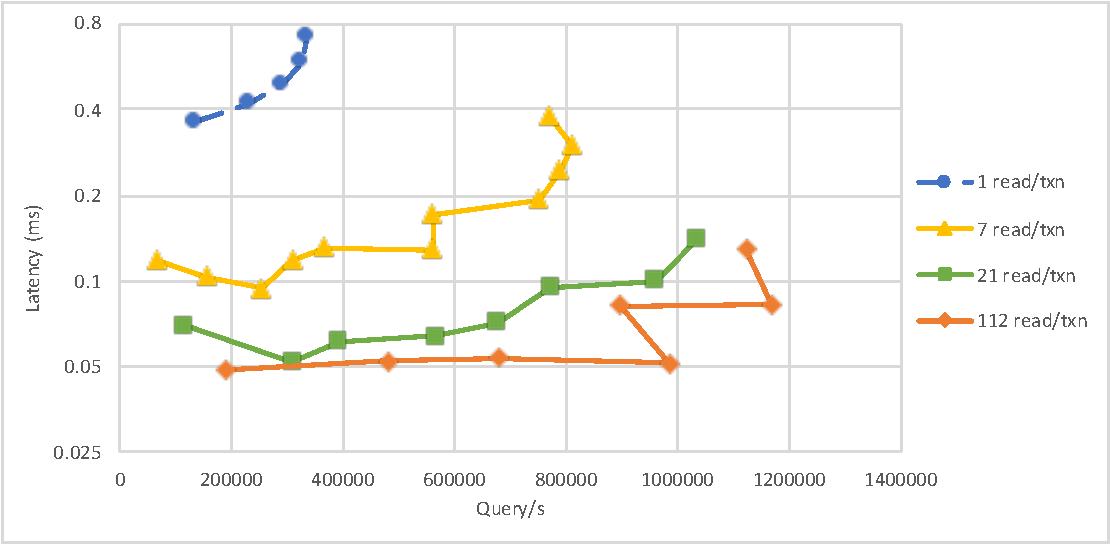
\includegraphics[width=.95\linewidth]{ops_per_txn_cut}
%	\caption{PotionDB performance when batching queries. Note that latency is in logarithmic scale.}
%	\label{fig:ops_per_txn}
%\end{figure}

\begin{figure}
	\centering
	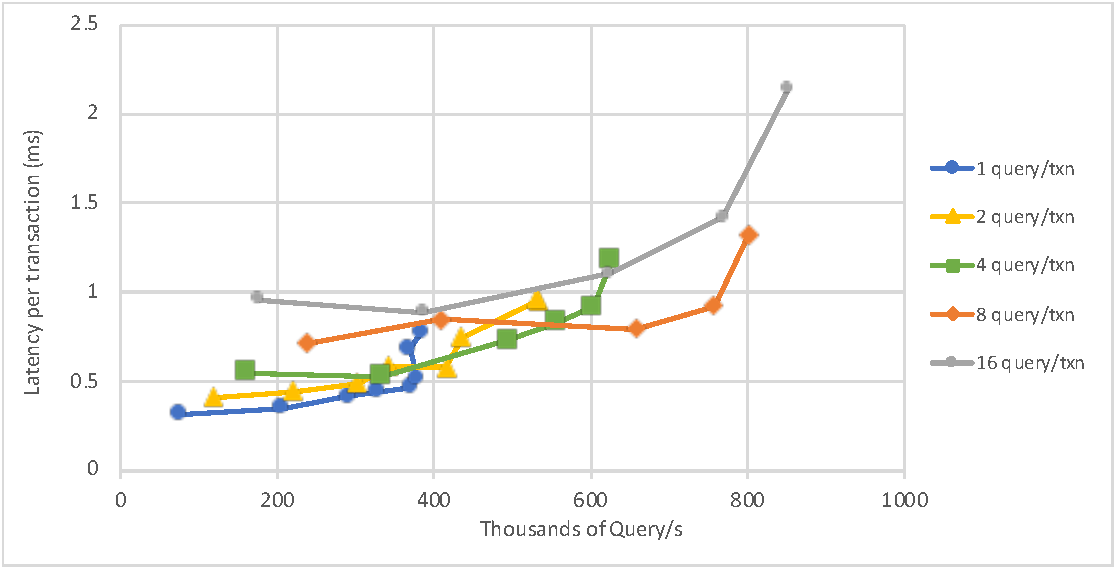
\includegraphics[width=.95\linewidth]{ops_per_txn_few_cut}
	\caption{PotionDB performance when batching queries. %Note that latency is in logarithmic scale.}
	}
	\label{fig:ops_per_txn}
\end{figure}

%\andre{Note: this graph is temporary - I'll have to repeat the tests with less clients and a few repetitions of the same executions. Also probably with lower values. When I first did this test it was more for curiosity than for really putting it here...}

Figure \ref{fig:ops_per_txn} shows how PotionDB scales in terms of query/s depending on how many queries are executed in each transaction.
As expected, as we increase the amount of queries per transaction, so does the latency, as there is more data to send, receive and process.
However, the beneficts for throughput are visible - comparing 1 query/txn with 8 query/txn, we can see the throughput more than double before the server saturates, and latency increase by less than double.
Increasing the number of queries/txn also leads to PotionDB saturating with less clients, as more time is spent on processing queries instead of waiting/switching clients, thus making better usage of machine resources.
%We can see that with batching PotionDB reaches its peak performance with a lower number of clients (high query/s with low latency), and is able to provide higher throughput with lower latency - up to 1.2M ops/s with batching compared to 0.36M ops/s without batching.

\subsubsection{CRDT Benchmark}

\andre{I didn't know what to title this}

We now evaluate how a single PotionDB server scales outside of the TPC-H scenario.
Namely we do a few benchmarks to determine the raw throughput of PotionDB when executing random operations, instead of specific queries or updates.

\begin{figure}
		\centering
	\begin{subfigure}{.535\linewidth}
		\centering
		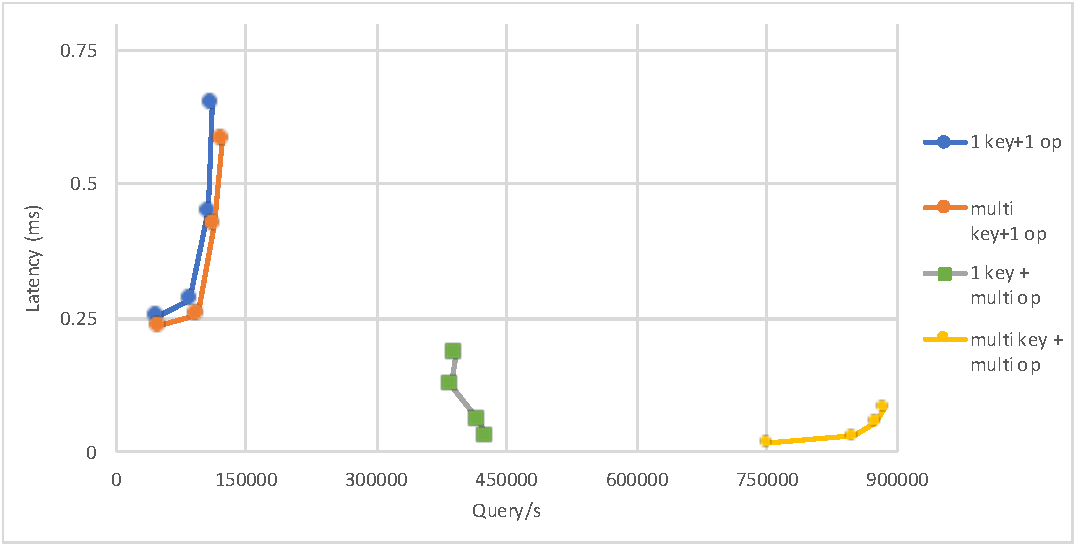
\includegraphics[width=.95\linewidth]{bench_read_cut}
		\caption{Read-only}
		\label{fig:bench_read}
	\end{subfigure}%
	\begin{subfigure}{.465\linewidth}
		\centering
		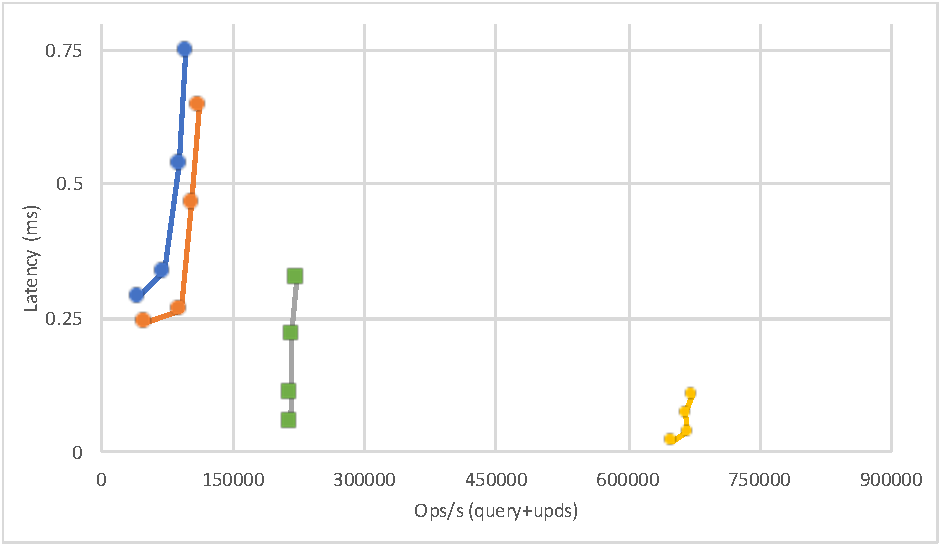
\includegraphics[width=.95\linewidth]{bench_update_cut}
		\caption{10\% update rate}
		\label{fig:bench_upd}
	\end{subfigure}
	\caption{Single server performance when executing random operations on set CRDTs. 1 key corresponds to a single CRDT shared between all clients, while multi key corresponds to multi CRDTs per client. 1/multi op refer to single or multi operation transactions.}
	\label{fig:bench}
\end{figure}

Figure \ref{fig:bench} contains results on the execution of benchmarks on set CRDTs.
Namely, figure \ref{fig:bench_read} concerns a read-only scenario, while \ref{fig:bench_upd} has a 10\% update rate.

Focusing on figure \ref{fig:bench_read}, it can be observed that increasing the number of operations per transaction greatly increases the throughput (up to 7x more in the tested scenario).
Increasing the number of CRDTs only seems to have a considerable effect when there's multiple operations in a transaction.
This may be due to the fact that a lookup operation in a set CRDT executes so quickly that most of the overhead may be in communication between threads or on converting data to the wire, thus not taking much benefict from the CRDTs being split across different partitions.

Considering figure \ref{fig:bench_upd}, considerably lower latencies can be observed when using multiple keys with only 1 operation per transaction.
Based on other tests we done, we can affirm that this difference is bigger the higher the rate of updates are.
This is due to the fact that updates must lock a partition, thus if different keys are used, and each client only manipulates one key at a time, some reads may be executed in parallel with updates, as long as it is for different partitions.
With a single key used by all clients, no concurrency is possible when an update is being executed.

The observed performance is worse than in a read-only scenario, 
which is specially noticeable in scenarios with multiple operations per transaction.
IThis is even more noticeable in the case with only one key, as the vast majority of transactions will include updates and thus the different clients end up having their transactions executed sequentially.
Having multiple keys eases this, as only partitions which get updated need to be locked, thus some concurrency is still possible.

\andre{This subsection VERY LIKELY needs to be rewritten/better thought of. Maybe even choose different data to show...}

%\subsection{Old Results}
%
%We first start by comparing the performance between running PotionDB in its intended mode, i.e., with views of global data, versus having each view only include data replicated locally.
%To distinguish between both, we call the former simply PotionDB and the later Local PotionDB.
%It is expectable for Local PotionDB to have worse performance, as most TPC-H queries concern data that is replicated across multiple replicas, which implies that clients need to contact multiple replicas to answer a single query in the case of local views.
%
%\begin{figure}
%	\centering
%	\begin{subfigure}{.5\linewidth}
%		\centering
%		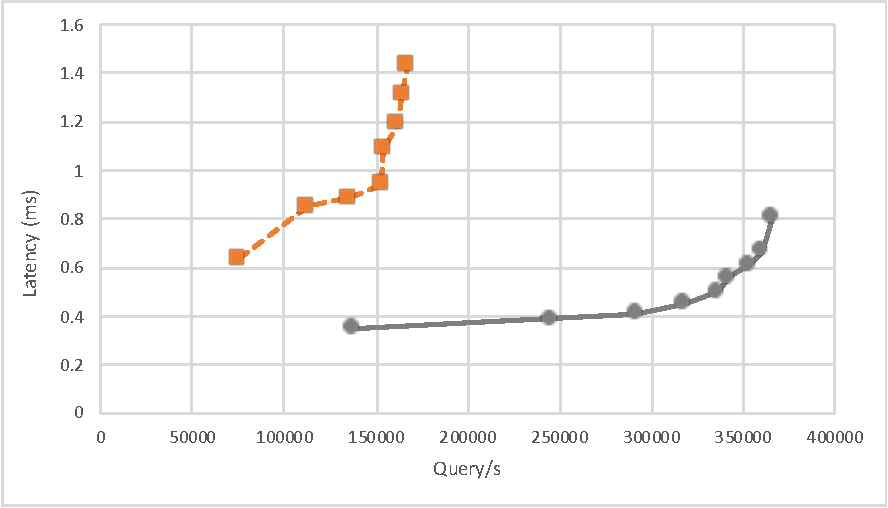
\includegraphics[width=.95\linewidth]{8_CPU_global_LQ_cut}
%		\caption{Global PotionDB}
%		\label{fig:global8CPU}
%	\end{subfigure}%
%	\begin{subfigure}{.5\linewidth}
%		\centering
%		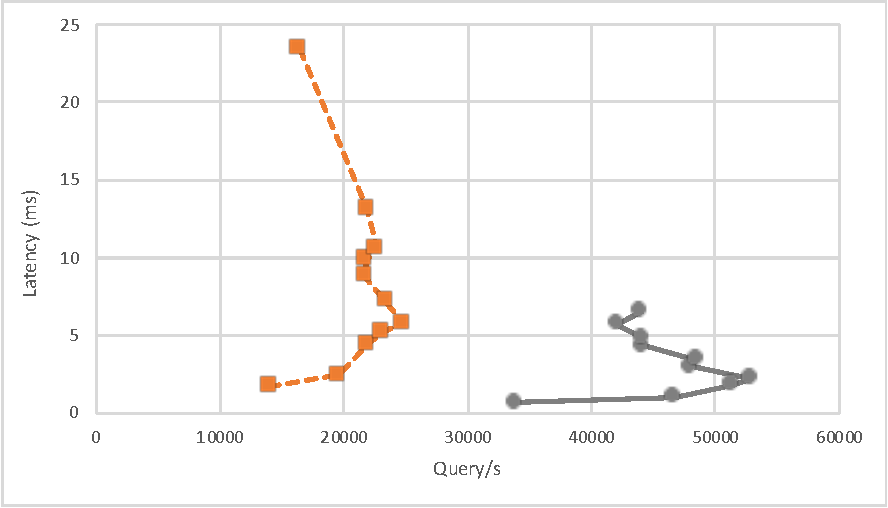
\includegraphics[width=.95\linewidth]{8_CPU_local_LQ_cut}
%		\caption{Local PotionDB}
%		\label{fig:local8CPU}
%	\end{subfigure}
%	\caption{Performance of PotionDB (left) with global indexes versus a version with local indexes (right). Square points represent the situation with both query clients and an update client, while circle is query only. Notice the difference in the scales between the graphs.}
%	\label{fig:8CPU}
%\end{figure}
%
%%\andre{Suggestions for graphs are more than welcome. Also, should instead of using Figure \ref{fig:global8CPU} and \ref{fig:local8CPU} use a single graph which contains both the local and global scenarios?}
%%
%%\begin{figure}
%%	\centering
%%	\begin{subfigure}{.5\linewidth}
%%		\centering
%%		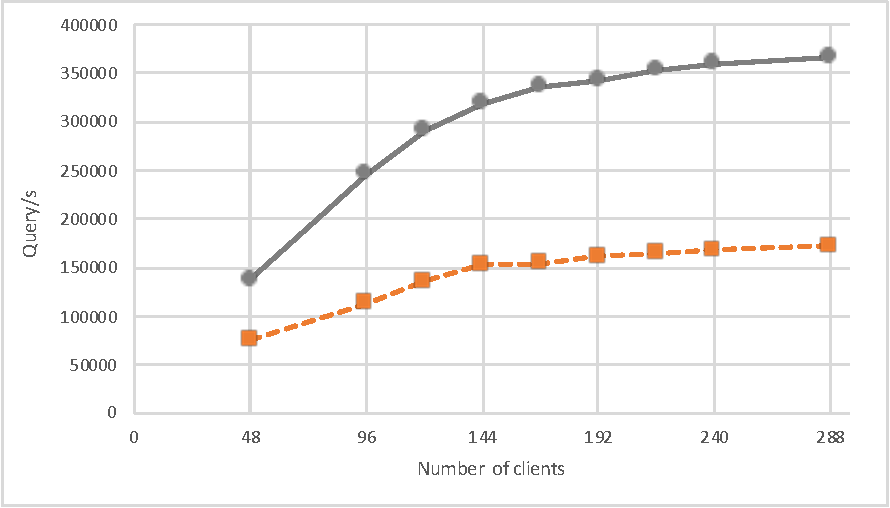
\includegraphics[width=.95\linewidth]{8_CPU_global_index_cut}
%%		\caption{Global PotionDB}
%%		\label{fig:global8CPU}
%%	\end{subfigure}%
%%	\begin{subfigure}{.5\linewidth}
%%		\centering
%%		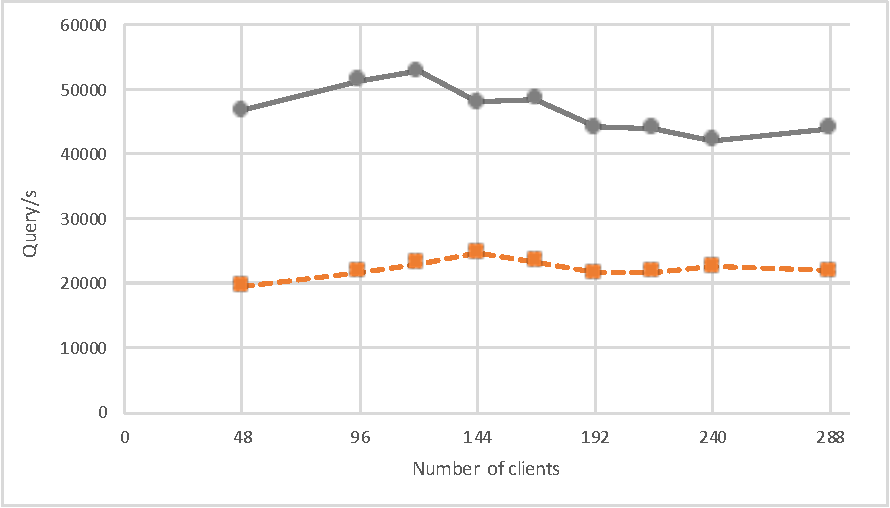
\includegraphics[width=.95\linewidth]{8_CPU_local_index_cut}
%%		\caption{Local PotionDB}
%%		\label{fig:local8CPU}
%%	\end{subfigure}
%%	\caption{Performance of PotionDB (left) with global indexes versus a version with local indexes (right). Square points represent the situation with both query clients and an update client, while circle is query only. Notice the difference in the y scale (query/s) between the graphs.}
%%	\label{fig:8CPU}
%%\end{figure}
%%
%
%\andre{TODO: Este texto é ainda o antigo!!!}
%
%Figure \ref{fig:global8CPU} and \ref{fig:local8CPU} show the results of experiments for, respectively, PotionDB and Local PotionDB in terms of query/s.
%There is at least two noteworthy points to be taken from the graphs.
%
%First, the number of queries that PotionDB can answer decreases to aproximately half when there are updates going on - this is expected, as due to causality PotionDB needs to ensure all reads of a transaction see the same version.
%This also implies that old object versions may need to be computed, which implies extra server work.
%
%Second, as expected, the local version has considerably lower performance than the global version, peaking its performance at a much lower number of clients (120 to be precise).
%In short this can be justified by considering that to answer a single query in the local version, multiple servers may need to be contacted. 
%To exemplify, consider the query "Top 10 product orders not yet shipped."
%This could be answered with a single Top-K CRDT read in the global scenario, but on the local scenario all servers need to be contacted as each server only knows of the orders done in its continent.
%Thus, the client has to wait for all servers to answer and then aggregate the results before moving to the next query.
%In other words, for some queries all servers need to reply to all clients and thus send/process more data, unlike with the global scenario in which each server is, in practice, dedicated to a subset of the clients.
%In conclusion, there is a performance gain to be obtained from having indexes of data replicated both locally and on other servers when there are queries that concern such data.

\section{Related Work}

%y [12, 18, 22, 29, 36, 44], an

%TODO: Veronica uses projection to improve queries, might be worth comparing to.

\andre{Self-critic: this is lacking a comparison to specific solutions. What I'm providing here is a more generic view on multiple topics relevant to PotionDB.}

Database systems can offer different levels of consistency, with solutions usually being labeled as either strong consistency or weak consistency.
Strong consistency systems \cite{spanner, slog, scatter, krikellas2010strongly, redblue, megastore} are easier to work with as they provide a total order for their transactions.
However, the CAP theorem \cite{cap} implies that availability may be compromised in case of network partitions. Furthermore, high latency is to be expected in geo-distributed scenarios as multiple datacenters need to be contacted in order to commit a transaction.
By relaxing the provided consistency guarantees, weak consistency systems \cite{dynamo, couchDB, cassandra, chainreaction, cops, riak} can provide low latency, high throughput and better fault tolerance.
However, concurrency conflicts make those solutions harder to work with.
Causal consistency is a sub-form of weak consistency that alleviates this problem, however anomalities can still be observed even with cross-object causality \cite{cops, burckhardt2013understanding}.

Both indexes and materialized views can speed up the execution of queries.
Indexes can provide quick access to a table or object using a non-primary key, and are often used by queries which require sorting or a given range of values.
Multiple systems implement indexes \cite{dynamo, couchDB, cassandra, megastore} and research on efficient usage and storage of those is a common research topic \cite{lee2020asymmetric, lisa, alex, bindex, slik}.
On the other hand, materialized views work as a cache for the result of a large query.
Materialized views can provide quick access to data that would take a long time to calcultate, and are often useful for analytic queries \cite{analyticdb}.
\andre{[I didn't find a proper reference for ``views being useful for analytic queries''. Suggestions?]}
However, maintaining views consistent and automatically updated is challenging \cite{oracleViews, chronocache, birds} and few systems implement them \cite{chronocache, marviq, estocada, couchDB, oracleViews, noria}, even though they can speed up queries considerably.
To the best of our knowledge, PotionDB is the first system to support materialized views in a geo-distributed, partially replicated scenario.

Geo-distributed scenarios imply high latency when acessing far away datacenters, which is required for strong consistency \cite{chronocache, slog, cops, lloyd2013stronger}. 
Network partitions are also a concern, as they may render strongly consistent systems unavailable.
Weak consistency can help avoid both problems, but lack the useful consistency guarantees provided by strong consistency.

\andre{I still need to find citations for partial replication. Any suggestion/starting point is more than welcome}

Partial replication allows to reduce storage costs and can even improve a system's performance (e.g., due to less operations to apply on each server), and are thus of interest for geo distribution.
The partitioning of the data must be carefully done by considering where each object may be relevant, as otherwise clients may need to access far away servers and thus experience high latency.
Many systems provide partial replication \cite{???}.
However, a problem not often analyzed in these kind of systems is that some analytic queries may need to consult objects sharded between different datacenters.
Without views, this process can be slow, specially when trying to provide a consistent snapshot of the database.
PotionDB tackles this problem by providing views that summarize partially replicated data and directly answer such queries.

Conflict-free Replicated Data Types, CRDTs \cite{crdt}, are replicated data types that guarantee state convergence, assuming all updates are eventually delivered.
Thus, they are often used in weakly consistent systems, e.g., Redis \cite{redisCRDT} and Riak \cite{riak}.
Some types of CRDTs have been introduced that can help with representing views of data, namely computational CRDTs \cite{computationalCrdt} and non-uniform CRDTs \cite{Cabrita17Nonuniform}.
The former computes some result over data (e.g., a sum), while the later focus on minimizing the information that needs to be replicated to correctly reply to queries (e.g.: a top-k CRDT doesn't need all entries to be replicated).
In PotionDB every object is a CRDT, and in particular we make usage of both computational and non-uniform CRDTs to support our views.

\andre{The comparisons to other systems are still unorganized, but at least there's already content.}

ChronoCache \cite{chronocache} is a middleware caching layer for geo-replicated databases which focus on combining multiple queries into one request and caching query results.
While the caching can speed up future requests, complex queries may still need to contact multiple servers and updates can invalidade the cache or else the clients read stale data.

AnalyticDB \cite{analyticdb} focus on optimizing analyctic queries. 
It separates write and read paths to prevent complex queries from slowing down writes. 
It also makes usage of indexes to speed up queries.
However, complex queries still take hundreds of milliseconds to execute and they may slow down other simpler queries.
They do not make usage of views.

SLOG \cite{slog} provides ACID transactions in a geo-distributed scenario.
They share one of PotionDB's insights - not all data is relevant everywhere and clients will often access data relevant in their region.
Thus, SLOG achieves low latency ACID transactions for transactions that can be served by a single datacenter.
However, unlike PotionDB, queries regarding data partitioned accross multiple datacenters has considerably higher latency.
We leverage on views of global data to prevent this.

ESTOCADA \cite{estocada} is a system designed to work with polystores and focus on taking advantage of each database's stronger points and make extensive usage of the materialized views provided on each.

%Preciso de rever este melhor (local/remoto?)
Marviq \cite{marviq} tackles the specific situation of efficiently providing a visualization (e.g., scatterplot) of a large data set.
While a more specific scenario than the one PotionDB aims for, it showcases similar challenges - large datasets that need to be sumarized and queried efficiently.
They make usage of materialized views to handle range queries on the datasets.

Magrino et. al. \cite{treaties} propose predictive treaties. 
The insight is that some computations can be expressed by treaties, and is possible to antecipate a range of how a value might change over time.
While this can lead to fast query replies and less duplicated data compared to views, since those treaties are not enforced as invariants, it is possible to read incorrect values.
It may also be unfeasable to predict changes for some data.

Noria \cite{noria} is a streaming data-flow system. 
It makes usage of views and partial data to provide fast query reply and reasonable memory usage.
While it features high throughput, it is only able to provide eventual consistency, which is tougher to work with than casual consistency.
There is also concerns on the performance of queries when a view needs to be rebuilt and data is sharded.

Dynamo \cite{dynamo} and Cassandra \cite{cassandra} both are eventually consistent databases (the latter can provide stronger consistency when needed).
Both provide indexes to speed up some queries but not materialized views, thus complex queries may need to access large amounts of objects.
CouchDB \cite{couchDB} provides both indexes and materialized views, however their views can only refer to data in one partition.

%Should prob make a general comparison to MongoDB/Cassandra/Dynamo

%Comparison to specific solutions?

%Geo-replication, partial-replication

%CRDTs?

%\section{[OLD]Related Work}
%
%Both strongly and weakly consistent solutions exist to support services that require geo replication of their data.
%%Strong consistency solutions like Spanner \cite{???} \comment{likely introduce others}
%%Some examples include, for strong, Spanner \cite{???} and ???; while for weak ??? and ???.
%Strong consistency solutions like Spanner \cite{spanner} and CockroachDB \cite{cockroachdb} provide the ilusion of a single replica, thus making it easier to provide a consistent view for clients.
%However, the CAP theorem \cite{cap} implies that availability may be compromised in case of network partitions, and high latency is expected as multiple datacenters need to be contacted for executing operations.
%Weak consistent solutions such as Dynamo \cite{dynamo} and COPS \cite{cops} can provide highly available, low latency operations, but providing a consistent view of the database to clients is challenging.
%Causal consistency is a sub-form of weak consistency that alleviates this problem, however anomalities can still be observed even with cross-object causality \cite{cops, burckhardt2013understanding}.
%
%Systems like Dynamo \cite{dynamo}, COPS \cite{cops} and CockroachDB \cite{cockroachdb} provide geo-replication.
%Dynamo provides partial replication, however reads and updates for multiple keys are done independently, thus there's no causal read of multiple reads.
%COPS provides causal+ consistency and supports transactions for reads, however it doesn't support neither partial replication or views.
%CockroachDB is strongly consistent and, thus, may fail due to network partitions, and does not provide partial replication.
% 
%CRDTs \cite{crdt} are replicated data types that guarantee state convergence, assuming all updates are eventually delivered.
%Thus, they are often used in weakly consistent systems, e.g., Redis \cite{redisCRDT} and Riak \cite{riak}.
%Some types of CRDTs have been introduced that can help with representing views of data, namely computational CRDTs \cite{computationalCrdt} and non-uniform CRDTs \cite{Cabrita17Nonuniform}.
%The former computes some result over data (e.g., a sum), while the later focus on minimizing the information that needs to be replicated to correctly reply to queries (e.g.: a top-k CRDT doesn't need all entries to be replicated).
%We leverage on both in our solution.
%
%Alternative solutions to provide global queries on partially replicated data includes using distributed processing systems like Pixida \cite{kloudas2015pixida} or Hourglass \cite{hourglass}.
%However, this impose challenges both consistency-wise, as well as in terms of latency and data transferred.
%The amount of data to be transfered is specially concerning, as if the underlyng systems only provide simple get operations, very high amounts of data may have to be transfered to reply to a small query like a top 10.
%PotionDB avoids this by having materialized views, which allows to have only the required data replicated in every server and thus reply to such query efficiently.
%%COPS doesn't support partial replication
%%Dynamo supports partial replication, but doesn't support views or consistent reads of multiple objects.
%%Start talking about partial replication
%%Mention some geo-distributed DBs, explain that they don't provide partial replication
%%CRDTs, non-uniform replication
%%Maybe at some point refers transactions
%%Refer alternative solution of pixida/parallel jobs.
%%Maybe mention views in consistent databases.
%%Hourglass is mentioned in Pixida paper.



\section{Conclusions}

\bibliographystyle{abbrv}
\bibliography{bib}

\null\newpage\null

\null\newpage\null

\section{Topics}

This contains the topics that were initially discussed during the first meeting and some afterthoughts.

\section{System overview}

\begin{itemize}
	\item System model
	\begin{itemize}
		\item Replicação parcial
	\end{itemize}
	\item System API
	\begin{itemize}
		\item "Create table"
		\item "Create view"
		\begin{itemize}
			\item CRDT não uniforme
			\item put numa table $\implies$ puts nas várias views
			\begin{itemize}
				\item consistência das views face aos dados - in sync
			\end{itemize}
		\end{itemize}
	\end{itemize}
	\item System description
	\begin{itemize}
		\item CRDT não uniforme
		\item Implementação de queries?
	\end{itemize}
	
\end{itemize}

\section{Implementation}

\section{Evaluation}

%- Dizer o que se vai avaliar.
%- Ter um gráfico com o que seria de esperar.

\section{Related Work}

\section{Conclusions}

\section{System overview}
Possiveis pontos mais detalhados?

\subsection{System model}

\begin{itemize}
	\item Network assumptions
	\item Client-server interaction (refer key-value store interface? Maybe refer this instead in System API?)
	\item Server-server interaction? (is it needed? We'll already touch this in Replication.)
	\item System guarantees
	\begin{itemize}
		\item CRDTs
		\item Consistency level	
	\end{itemize}
	\item Replication
	\item Async
	\item Op-based
	\item Maintains consistency, i.e., transaction level based.
	\item Partial (system admin defined, each server only has a subset of the data based on topics. Potencially some data can be replicated everywhere)
\end{itemize}

\subsection{System API}

\begin{itemize}
	\item Basically how can we translate a problem to sql-like operations
	\item Create table
	\item Create view
	\item Updates (incluir problema de consistência de views/dados)
	\item Queries (incluir aqui problema de os CRDTs não uniformes precisarem de mais dados? Ou na zona da view?)
\end{itemize}

\subsection{System description}

\begin{itemize}
	\item Structure? Maybe that's for implementation? How much detail?
	\begin{itemize}
		\item Internal partitioning vs external partitioning? Capaz de não ser boa ideia...	
	\end{itemize}
	\item CRDTs and non-uniform CRDTs?
\end{itemize}

\andre{I ended up describing the topics of system description in other subsections, apart from Structure. I don't recall going into much detail of what a CRDT is, but that shouldn't be necessary anyway.}

\section{Implementation}

\begin{itemize}
	\item Go
	\item Transactions (TM/Mat?)
	\item Replication (RabbitMQ and other stuff?)
	\item Communication (protobufs. Also worth noticing the compability with existing AntidoteDB clients)
	\item CRDTs (version management at least)
\end{itemize}

\andre{A good part of the implementation is already included in other sections, at least indirectly. Mainly Replication and to an extent Transactions/Communication. We need to decide what really is important to refer in the "implementation" section.}

\end{document}
